\documentclass{ntuthesis}


%\usepackage{xeCJK}
%%%%%%%%%%%%
\usepackage{bbold}
%\usepackage[backend=biber]{biblatex}
\newcommand{\citep}{\cite}
\usepackage{cite}
\usepackage{subfigure}
\usepackage{xcolor}
\newcommand{\be}{\begin{eqnarray}}
\newcommand{\ee}{\end{eqnarray}}
\usepackage{amsfonts}
\usepackage{bbm}
\usepackage{amsmath,leftidx}
\usepackage{graphicx}
\usepackage{times}
\usepackage{CJK}
\usepackage{color,colortbl}
\usepackage[normalem]{ulem}
\usepackage{hyperref}
%\usepackage[sorting=none]{biblatex}
\usepackage{indentfirst}

%%%%%%%%%%%

\usepackage{times}

\usepackage{verbatim}
\usepackage{color}
\usepackage{url}
\usepackage{graphicx}
\usepackage{array}
\usepackage{wallpaper}
\usepackage{hyperref}
\usepackage[printwatermark]{xwatermark}
\usepackage{graphicx}
\graphicspath{ {./Figures/} }
\usepackage{tikz}

% Using the tex-text mapping for ligatures etc.
\defaultfontfeatures{Mapping=tex-text}

% Set the default fonts
\setmainfont{Times New Roman}
\setCJKmainfont[AutoFakeBold=true,AutoFakeSlant=true]{標楷體}
%\setCJKmainfont[BoldFont={粗楷體},ItalicFont={斜楷體}]{標楷體}

\ifdefined\firstpage
  \ifdefined\withwatermark
    \newsavebox\mybox
    \savebox\mybox{\tikz[opacity=0.5]\node{\includegraphics{watermark.pdf}};}
    \newwatermark*[allpages,xpos=6.1725cm,ypos=10.5225cm,scale=0.5]{\usebox\mybox}
  \fi

  % digital object identifier
  \ifdefined\withdoi
    \insertdoi
  \fi
\fi

\makeatletter
\AtBeginDocument{
  \hypersetup{
    pdftitle={\@titleen},
    pdfauthor={\@authoren},
    pdfsubject={\@typeen{} \@classen},
    pdfkeywords={\@keywordsen}
  }
}
\makeatother

% Your information goes here
% author: Tz-Huan Huang [http://www.csie.ntu.edu.tw/~tzhuan]

% ----------------------------------------------------------------------------
% "THE CHOCOLATE-WARE LICENSE":
% Tz-Huan Huang wrote this file. As long as you retain this notice you
% can do whatever you want with this stuff. If we meet some day, and you think
% this stuff is worth it, you can buy me a chocolate in return Tz-Huan Huang
% ----------------------------------------------------------------------------

% Syntax: \var{English}{Chinese}
\university{National Taiwan University}{國立臺灣大學}
\college{College of Science}{理學院}
\institute{Department of Physics}{物理學系}
\title{Study of Kitaev Spin Liquids using Symmetric Tensor Network
}{藉由對稱性張量網路探討Kitaev自旋液體}
\author{Yu-Hsueh Chen}{陳昱學}
\studentid{R09222009}
\advisor{Ying-Jer Kao, Ph.D.}{高英哲 博士}
\defenseyear{2021}{109}
\defensemonth{April}{4}
\defenseday{28}
\doi{doi:10.6342/NTU20XXXXX}
\keywords{keyword}{關鍵字}


\begin{document}

\frontmatter

\makecover

\ifdefined\excludefirstpage

  \ifdefined\withwatermark
    \newsavebox\mybox
    \savebox\mybox{\tikz[opacity=0.5]\node{\includegraphics{watermark.pdf}};}
    \newwatermark*[allpages,xpos=6.1725cm,ypos=10.5225cm,scale=0.5]{\usebox\mybox}
  \fi

  % digital object identifier
  \ifdefined\withdoi
    \insertdoi
  \fi
\fi

\makecertification

\begin{acknowledgementszh}
感謝\ldots
\end{acknowledgementszh}

\begin{acknowledgementsen}
I'm glad to thank\ldots 
\end{acknowledgementsen}

\begin{abstractzh}
本論文

\bigbreak
\noindent \textbf{關鍵字:}{\, \makeatletter \@keywordszh \makeatother}
\end{abstractzh}

\begin{abstracten}
In this thesis, we ...
\bigbreak
\noindent \textbf{Keywords:}{\, \makeatletter \@keywordsen \makeatother}
\end{abstracten}

\begin{comment}
\category{I2.10}{Computing Methodologies}{Artificial Intelligence --
Vision and Scene Understanding} \category{H5.3}{Information
Systems}{Information Interfaces and Presentation (HCI) -- Web-based
Interaction.}

\terms{Design, Human factors, Performance.}

\keywords{Region of interest, Visual attention model, Web-based
games, Benchmarks.}
\end{comment}


\tableofcontents
\listoffigures
\listoftables

\mainmatter

% Your thesis goes here
%\chapter{Introduction}
\label{c:intro}

Attention plays an important role in human vision. For example, when
we look at an image, our eye movements comprise a succession of {\em
fixations} (repetitive positioning of eyes to parts of the image)
and {\em saccades} (rapid eye jump). Those parts of the image that
cause eye fixations and capture primary attention are called {\em
regions of interest} (ROIs). Studies in visual attention and eye
movement have shown that humans generally only attend to a few ROIs.
Detecting these visually attentive regions in images is challenging
but useful in many multimedia applications, such as automatic
thumbnail cropping, object recognition, content-based image
retrieval, adaptive image compression and automatic browsing in
small-screen devices.

Many algorithms have been proposed for automatic ROI detection in
images. Unfortunately, these methods were often evaluated only on
specific and small data sets that are not publicly available. The
lack of published {\em benchmarks} makes experiments non-repeatable
and quantitative evaluation difficult. However, as recommended by
the latest ACM SIGMM retreat, repeatable experiments using published
benchmarks are important for advancing the multimedia research
field~\cite{Rowe:2005:ASR}.

\begin{figure}
\centering
\includegraphics[width=\textwidth]{model_and_LG}
\caption{LG-property}
\label{fig:LG_property}
\end{figure}

\begin{figure}
\centering
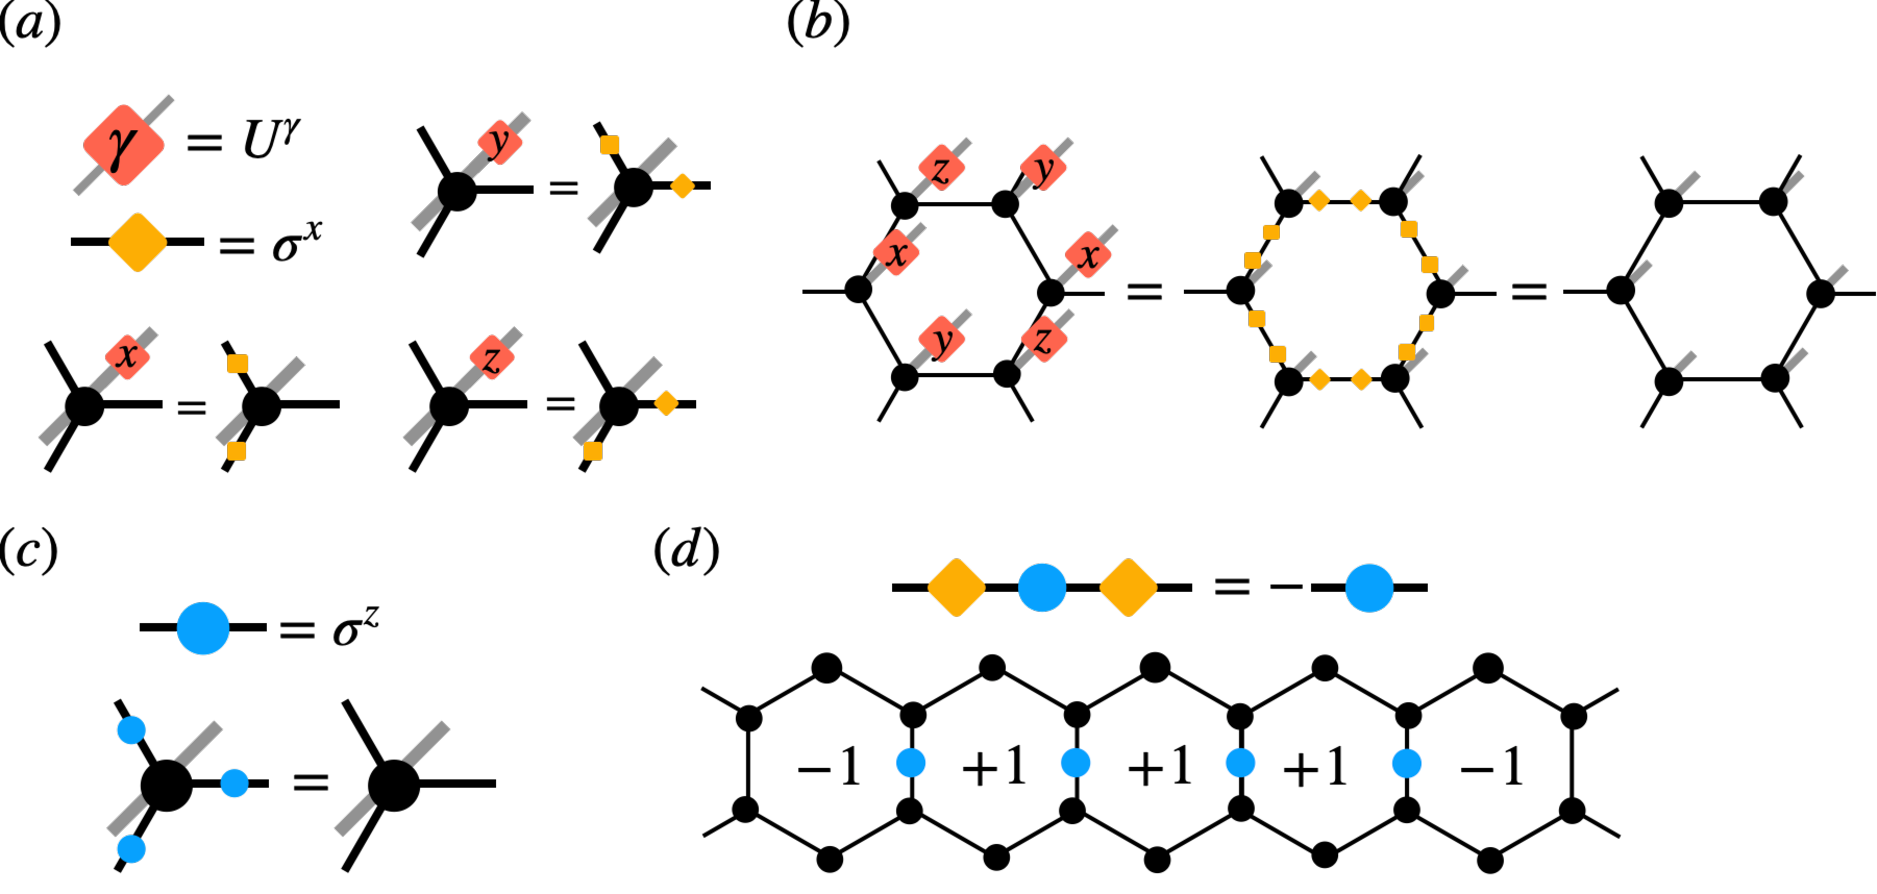
\includegraphics[width=\textwidth]{LG_property}
\caption{LG-property}
\label{LG_property}
\end{figure}



\begin{table}[t]
\begin{center}
\begin{tabular}{lcc}

\hline
                    &  {\small Itti's method}     & {\small Fuzzy growing}    \\
\hline
{\small Precision}           &  0.4475    & 0.4506 \\
{\small Recall}              &  0.5515    & 0.5542 \\
\hline

\end{tabular}
\caption[Evaluation of FOA sets]{\small Evaluation of FOA sets. } \label{t:FOA}
\end{center}
\end{table}

\chapter{Introduction}
\label{c:intro}

QSL review:
\cite{Savary_2016, RevModPhys.89.025003, Broholmeaay0668}

Topological phase:
~\cite{Wen1989,Wen1990}

Nontrivial quasiparticle statistics:
~\cite{wen_1990,Wen1993,KITAEV20062, Bais_2012, Zhang_2012}.

topological entanglement entropy~\cite{ Kitaev2006, Levin2006,Xie_2010}, and  entanglement spectrum~\cite{Haldane_2008,Pollmann_2010,Turner_2011}.

Tensor Network:
\citep{2008_PEPS}


Kitaev original work:
\citep{Kitaev2006}

Spin-1/2 experiment:
\citep{PhysRevLett.108.127203, doi:10.1146/annurev-conmatphys-020911-125138,doi:10.1146/annurev-conmatphys-031115-011319, Winter_2017, PhysRevB.90.041112, Kasahara_2018}

Spin-1 theory:
\citep{Baskaran_2008,PhysRevB.99.104408, PhysRevB.98.214404}

Spin-1 microscopic mechanism:
\citep{PhysRevLett.123.037203}

Spin-1 numerical study:
Exact solution: \citep{2018_exact_spin1},
DMRG: \citep{2018_Kitaev_QSL,PhysRevB.102.121102,PhysRevResearch.2.022047,PhysRevResearch.3.013160}
iPEPS: \citep{2020-spin-one-kitaev,lee2020anisotropy}

Loop gas states (spin-1/2):
\citep{spin_one_half, non-AbelianTO_2020, Lee_2020}

Transfer Matrix:
\citep{2015_Zauner,Haegeman_2015,1972_Lieb} 

Z2-injective PEPS:
\citep{2011_Norbert_Ginjective}



Anyon Condensation:
\citep{2009-PRB-Condensate-induced, Norbert_Schuch_2013,Haegeman_2015, 2017_anyon_condensates
, 2017_Z4_anyon, 2017_sym_induced,2018_Chen_Boson_condensation, Zhang_2019}

MES: 
\citep{2012-PRB-Oshikawa-MES}


\chapter{Symmetric Tensor Network}

\section{$\mathbb{Z}_2$-injective PEPS, Anyon, and Minimally Entangled State}
\label{sec:Z2PEPS}

A translational invariant projected entangled pair states (PEPS) \citep{2008_PEPS} is a tensor network (TN) wave functions that can be written as a tensorial trace over the virtual indices of a PEPS tensor $A^i_{\alpha\beta\gamma\delta}$ with the physical index $i$ and virtual indices $\alpha, \beta, \gamma, \delta$:
\begin{equation}
\left|\psi_A\right\rangle=\sum_{i_1,\ldots,i_N} \operatorname{tTr}\left(A^{i_1}A^{i_2}\ldots A^{i_N}\right)|i_1, i_2,\ldots,i_N\rangle.
\end{equation}

The PEPS tensor can be regarded as a linear map from the virtual to the physical dimension: $P(A) = \sum_{i \alpha \beta \gamma \delta} A^i_{\alpha\beta\gamma\delta} |i\rangle_p \langle \alpha\beta\gamma\delta|_v$. 
%
In this perspective, the injective PEPS means that there exists a left inverse $P(A)^{-1}$ such that $P(A)^{-1} P(A) = \mathbb{1}_v$. In other words, for any injective PEPS $A$, we can find a tensor $A^{-1}$ such that  by tracing out the physical index with $A$, it is an identity acting on the virtual dimensions (Fig.\ref{fig:injectivePEPS}(a)). Physically, it means that the virtual and physical space has a one-to-one correspondence. 
%
For any PEPS tensor, there exists a local frustration-free parent Hamiltonian such that the PEPS wave functions is its ground state.
%
If the tensor is injective, its PEPS wavefunctions is the unique ground state of the parent Hamitlonian (Fig.~\ref{fig:injectivePEPS}(b)) \citep{2011_Norbert_Ginjective}. Besides, one can create a localized excitation by perturbing one PEPS tensor such that its energy differs from the ground state only in some local region.


\begin{figure}[t]
\centering
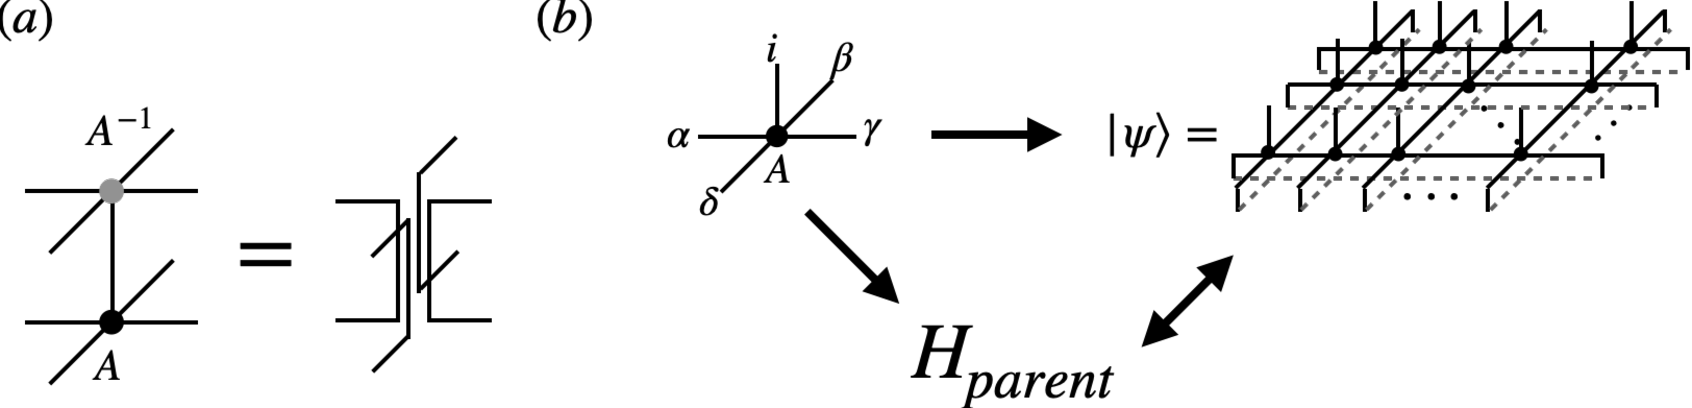
\includegraphics[width=\linewidth]{injectivePEPS}
\caption{(a) A tensor $A$ is injective if it has an inverse $A^{-1}$ such that by tracing out the physical index with $A$, it is an identity acting on the virtual dimensions. (b) If the tensor is injective, there exists a local patent Hamiltonian such that the corresponding PEPS wave functions is its unique ground states.}
\label{fig:injectivePEPS}
\end{figure}

Let's now turn to the PEPS that supports topologically non-trivial excitations.
If the PEPS tensor $A$ is invariant under the global $\mathbb{Z}_2$ symmetry: $A(u_g \otimes u_g \otimes u_g^\dagger \otimes u_g^\dagger) = A $, where $u_g$ is a representation of the group $\mathbb{Z}_2 $ with $g \in \{I, Z\}$ (Fig.~\ref{fig:Z2injectivePEPS}(a)), we say that $A$ is $\mathbb{Z}_2$-invariant.
%
A $\mathbb{Z}_2$-injective PEPS is a $\mathbb{Z}_2$ invariant PEPS existing a left pseudoinverse $P(A)^{-1}$ such that $P(A)^{-1} P(A) = \Pi_v$ where $\Pi_v$ is a projector onto the invariant subspace.
%
In other words, the global $\mathbb{Z}_2$ symmetry is the only global symmetry for a $\mathbb{Z}_2 $-injective PEPS.
%
For a $\mathbb{Z}_2$-injective PEPS, the ground state subspace of the parent Hamiltonian is no longer unique, but spanned by the two non-contractible loop operators, $(u_g^{\otimes L_x}, u_h^{\otimes L_y} ),\  \forall g,h \in \{{I}, Z\}$ acting on the states, which we denote as $|\psi_A(g,h)\rangle$ (Fig.~\ref{fig:Z2injectivePEPS}(c)). 
%
This arises from the fact that the non-contractible loop operators can always be deformed using the pulling-through condition (Fig.~\ref{fig:tm_sym}(a)) and the parent Hamiltonian cannot detect these loop operators locally. 
%


\begin{figure}[t]
\centering
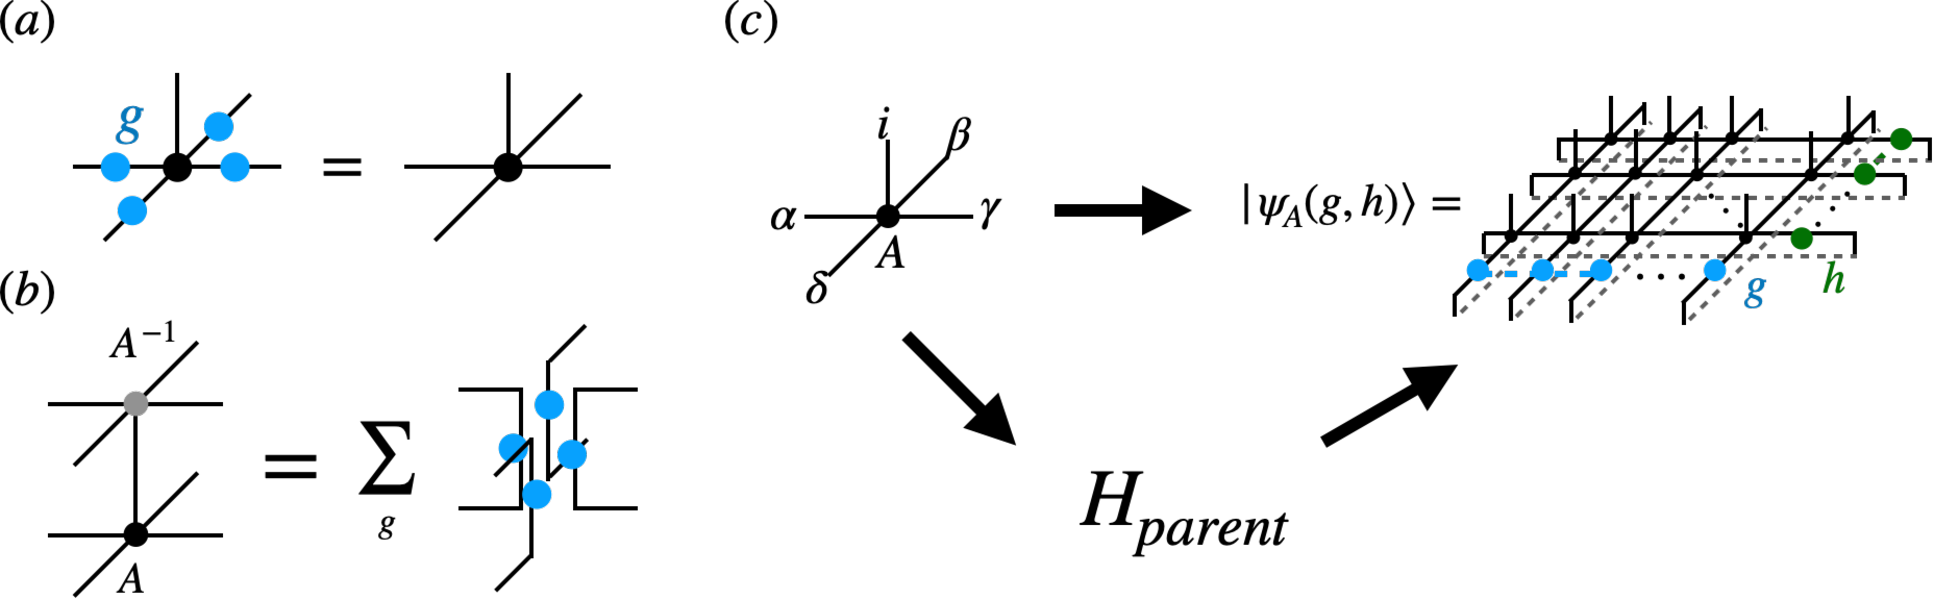
\includegraphics[width=\linewidth]{Z2injectivePEPS}
\caption{A $\mathbb{Z}_2$-injective PEPS is invariant under $A(u_g \otimes u_g \otimes u_g^\dagger \otimes u_g^\dagger) = A $, where $g \in \{{I}, {Z}\}$ (a) and there exists a $A^{-1}$ such that $A^{-1}A$ is the projection onto the invariant subspace (b). (c) For any $\mathbb{Z}_2$-injective PEPS $A$, we can construct a parent Hamiltonian such that its ground state subspace on the torus is spanned by $|\psi_A(g,h)\rangle, \,  \forall g,h \in \{{I}, Z\}$. }
\label{fig:Z2injectivePEPS}
\end{figure}

The $\mathbb{ Z}_2$-injective tensor naturally supports anyonic excitations that cannot be created locally on the physical space. 
%
For example, a flux excitation can be created by attaching a string of $u_g,\ g\in \{{I}, Z\}$ on the virtual dimension (Fig.~\ref{fig:anyon_MES}(a)).
%
A charge excitation can be created by acting an operator $R_\alpha$ on the virtual dimension. Here $R_\alpha$ transforms non-trivially under the group action $R_\alpha u_g = \chi_\alpha(g) u_g R_\alpha$, where $\chi$ is the character and $\alpha$ designates the irreducible representation of  $\mathbb{Z}_2$ (Fig.~\ref{fig:anyon_MES}(b))~\citep{2011_Norbert_Ginjective,2017_anyon_condensates}. 


\begin{figure}[t]
\centering
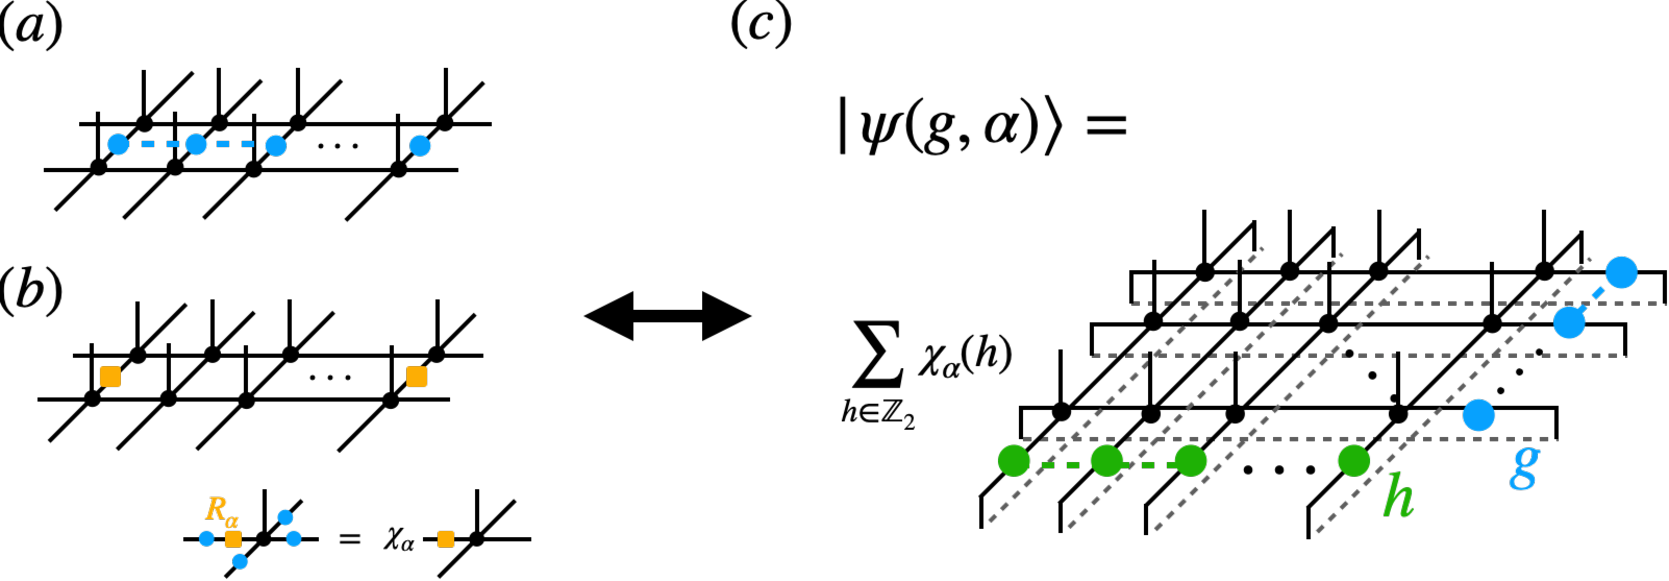
\includegraphics[width=\linewidth]{anyon_MES}
\caption{(a) A flux anyon is constructed by attaching a string of $u_g$. (b) A charge anyon is created by applying $R_\alpha$ on the virtual dimension, where $R_\alpha$ transform non-trivially under the group action. (c) The MES basis relating to anyon excitations can be constructed through $|\psi_A(g, \alpha)\rangle = \sum_{h \in \mathbb{Z}_2 }\chi_\alpha(h) |\psi_A(g,h) \rangle$. }
\label{fig:anyon_MES}
\end{figure}

Ground states subspace and the anyonic excitation are closely related, and we can construct a special ground state basis, the minimally entangled states (MESs), to reflect the anyonic excitation of the topological phases \cite{2012-PRB-Oshikawa-MES}. 
%
Basically, the MES basis can be obtained by creating a pair of anyons on a torus, wrapping them around a closed non-contractable loop, and finally annihilating them. 
%
To be specific, a MES is the eigenstate of the Wilson loop operator with a definite type of anyon excitation, and hence we can construct the MESs in the ground state subspace by  $|\psi_A(g, \alpha)\rangle = \sum_{h \in \mathbb{Z}_2 }\chi_\alpha(h) |\psi_A(g,h) \rangle$, with $g\in \{{I}, Z\}$ (Fig.~\ref{fig:anyon_MES}(c)). 
%
We then follow the same notation in Ref.~\cite{Norbert_Schuch_2013} to denote $g = {I} (Z)$ as 0($\pi$)-flux and the parity $\alpha $, as even (trivial) and odd (non-trivial).   
%
The four MESs $|I\rangle ,|e \rangle, |m \rangle, |\epsilon\rangle $ then correspond to  $|\psi_A(0,e)\rangle,|\psi_A(0,o)\rangle,|\psi_A(\pi,e)\rangle,|\psi_A(\pi,o)\rangle $, respectively.

The complete picture about the ground state subspace, anyon, and MES suggest that $\mathbb{Z}_2$-injective PEPS forms a natural framework to represent topologically ordered system. However, it is shown that a $G$-injective PEPS does not guarantee a topologically ordered phase, as the system can be driven into a topologically trivial phase by a physical deformation of the local tensor~\cite{Norbert_Schuch_2013,Haegeman_2015, 2017_anyon_condensates, 2017_Z4_anyon, 2017_sym_induced,2018_Chen_Boson_condensation, Zhang_2019}. 
%
In the next section, we will introduce transfer matrix, the central object in the tensor-network formalism that can be used to distinguish topological phase.



\section{Transfer Matrix}
Once the PEPS wave functions is obtained, the topological property and low-lying excitations can be studied by considering its normalization, which is encoded in the one-dimensional transfer matrix (TM) $\mathbb{T}$ (Fig.~\ref{fig:tm_cylinder}(a)).  
%
In what follows, we consider two different settings of the system: long cylinder and infinite plane. While those two cases are equivalent in the thermodynamic limit, the topological property is more straightforward to elaborate in the long-cylinder setting. On the other hand, the infinite-plane setting induces fresh notion about detecting topological phases using ``virtual order parameters'' and is computationally economical to extract low-energy dispersion.

\subsection{Long-Cylinder Setting: MES Overlap}
\label{subsec:long-cylinder}


As discussed in Sec.~\ref{sec:Z2PEPS}, we can always obtain four MESs by attaching two infinite string operators on the virtual Hilbert space. However it does not guarantee that those MESs are linearly independent or even a physically normalizable state. For instance, if the charge MES is identical to the vacuum MES, i.e., $\langle e| I \rangle = 1$, the ground state degeneracy may not be four anymore, and thus the system may not belong to $\mathbb{Z}_2$ topological order. Physically, this means that the charge anyon in the $\mathbb{Z}_2$ spin liquid phase condense to the ground state, as wrapping a charge pair around a non-contractable loop and annihilating them cannot produce a linearly independent state from the original ground state. Besides, the charge condensation will be accompanied by the confinement of the flux anyon, i.e., $\langle m | m \rangle = 0$ \citep{2009-PRB-Condensate-induced, 2017_anyon_condensates}.
%

\begin{figure}[t]
 \centering
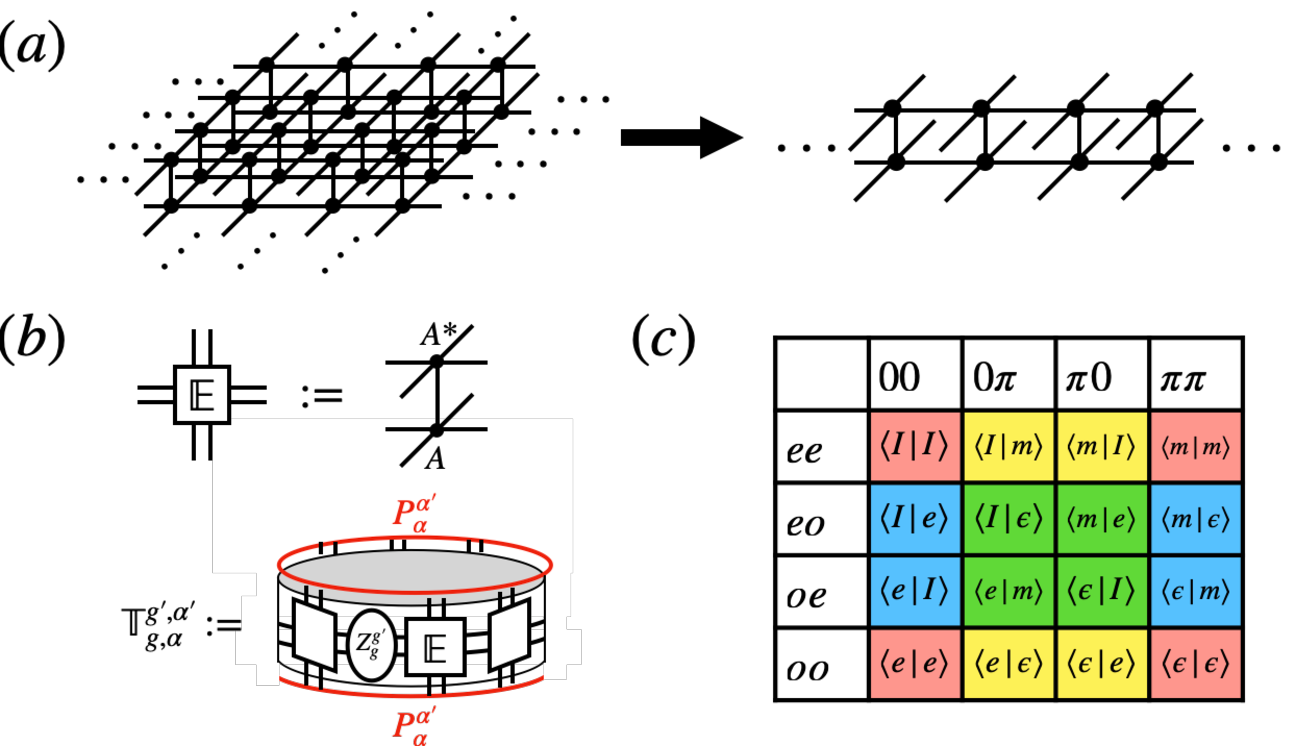
\includegraphics[width=\linewidth]{tm_cylinder}
\caption{(a) Overlap of two-dimensional infinite PEPS states can be regarded as a one-dimensional transfer matrix. (b) A double tensor is formed by contracting  tensor $A$ on a lattice site $a$ with its adjoint tensor $A^*$ over the physical index. (c) Sixteen blocks of the transfer matrices.}  
\label{fig:tm_cylinder}
\end{figure}

From the above argument, one can realize that the overlaps of MESs should be examined to nail down the phase for any $\mathbb{Z}_2$-injective PEPS, and it is natural to consider the transfer matrix defined on the long cylinder. 
%
To compute $\mathbb{T}$, we first form a double tensor  $\mathbb{E} $ (Fig.~\ref{fig:tm_cylinder} (b)) by contracting the physical indices of $\mathbb{Z}_2$-invariant PEPS $A$ and its adjoint $A^*$,
 $\mathbb{ E}  \equiv \sum_s ( A^s_{i,j,k,l} ) \times ( A^s_{i',j',k',l'} )^* $. 
%
The corresponding  transfer  matrix  is given by 
\begin{equation}
\mathbb{ T}  \equiv  \operatorname{tTr} ( \mathbb{E}^1  \mathbb{E}^2 \cdots \mathbb{E}^{N_x}   ). 
\end{equation}
%
The  minimally entangled topological sectors belonging to the quasi-particles can be obtained by inserting the string operator $Z_g = u_Z^g , (g=0,1)$  along the cylinder direction and choosing the projector $P_{\alpha}$ ($\alpha=$ even, odd) in either the bra or ket.
%
This gives 16 blocks of transfer matrices defined as (Fig.~\ref{fig:tm_cylinder}(b))
\begin{equation}
\mathbb{ T}_{\langle a|b \rangle} = \mathbb{ T}_{g,\alpha}^ {g',\alpha'}  \equiv  P_{\alpha}^ {\alpha'}  \big[ \operatorname{tTr} ( \mathbb{ E}^1  \mathbb{ E}^2 \cdots \mathbb{ E}^L  {Z}_g^{g'} )  \big]  P_{\alpha}^ {\alpha'}. 
\end{equation}
Here $ a = (g, \alpha) $ and $ b = (g', \alpha') $ with $g$ ($\alpha$) and $g'$  ($\alpha'$) label the string  (parity) operator in the ket and bra layer. 
%
Note that we refer the transfer matrix for a given block as ${\langle a | b \rangle}$ to simplify the notation in Fig.~\ref{fig:tm_cylinder}(c).


The transfer matrices can be further divided into four types:
 (a) $\alpha = \alpha'$ and $g=g'$ corresponding to the regular TM computing the norm of the MES, ${\langle a | a \rangle}$, with $ a = I,e,m, \epsilon $ (red color in Fig.~\ref{fig:tm_cylinder}(c)), 
 (b) $\alpha \neq  \alpha'$ and $g=g'$ corresponding to the mixed TMs measuring the charge difference between the bra and ket (blue), 
 (c) $\alpha =  \alpha'$ and $g \neq g'$ corresponding to the mixed TMs measuring the flux difference between the bra and ket  (yellow), 
 (d) $\alpha \neq  \alpha'$ and $g \neq g'$ corresponding to the mixed TMs measuring the both charge and flux (fermion) difference between the bra and ket (green).  
%
In the thermodynamic limit $N_x \rightarrow \infty$, the largest eigenvalue $\lambda_{\langle a|b \rangle}$  of  $\mathbb{ T}_{\langle a|b \rangle}$ encodes the overlap of the two MESs: 
%
If $\lambda_{\langle a|b \rangle} < 1$, then $\langle a|b \rangle = \lambda_{\langle a|b \rangle} ^{N_y} \rightarrow 0$ and the two MES are orthogonal; similarly, $\lambda_{\langle a|b \rangle} = 1$ means the two MES are the same. 
%
Therefore, in the $\mathbb{Z}_2$ topological order phase, the dominant eigenvalues of the regular TM are equal to one as $N_x \rightarrow \infty$ while the dominant eigenvalues of the other three mixed TM are less then one.
%
Nonetheless, as we will demonstrate at the end of this section, by tuning the wave function without spoiling the $\mathbb{Z}_2$-injectivity, it is possible to drive the system from a topological ordered phase to a topological trivial phase through the condensation of anyons. In this context, the classification in Fig.~\ref{fig:tm_cylinder}(c) is inappropriate.


%
It is also possible that an anyon can transmute into another type of anyon. 
%
For example, when the $D(\mathbb{Z}_4)$ quantum double model is continuously deformed to the toric code or the double semion model, some of the anyons distinct in the $D(\mathbb{Z}_4)$ phase can be identified as the same~\cite{2017_anyon_condensates, 2017_Z4_anyon}. 
%
Similarly, in the case of the $\mathbb{Z}_2$-injective PEPS, we can ask which anyons we can identify as the same.  
%
Since the TM is periodic around  the cylinder, we can label the states with the momentum quantum number.
%
Interestingly, it has been shown in Ref.~\citep{Haegeman_2015} that the momentum quantum number of $|\epsilon\rangle$ will be shifted by half a spacing, i.e., $k = 2\pi(n+\frac{1}{2})/L$, where $n = 0,\ldots ,L-1$ and $L$ is the circumference of the cylinder. 
%
This momentum polarization~\citep{2013_momentum_polarization} makes $|\epsilon\rangle$ impossible to become other MESs.
 %
This makes sense in the anyon condensation picture that fermion can never condense (corresponds to $|\epsilon \rangle \neq |I\rangle$), which has been proven in the more general case ~\citep{2017_anyon_condensates}.
 %
Discarding the possibility that  $|\epsilon\rangle$ becomes $|e\rangle$ or $|m\rangle$, we are left with the only choice to identify $|e\rangle$ and $|m\rangle$ as the same state. 
 %
 As we will see in Sec~\ref{sec:star_lattice}, the identification of $|e\rangle$ and $|m\rangle$ can be understood as the transition from the Abelian  to non-Abelian topological orders.

\subsubsection{Gauge-Symmetry Preserved HOTRG}
%\label{subsubsec:GSP-HOTRG}

Before analyzing the topological transition, we first introduce the numerical technique we develop, the gauge-symmetry preserved higher-order tensor renormalization group (GSP-HOTRG), to compute the overlap of the transfer matrices. This coarse-graining method extends the idea in Ref.~\cite{GSPRG_2014} to approximate the TM on the long cylinder with well preserved gauge symmetry.

\begin{figure}[t]
 \centering
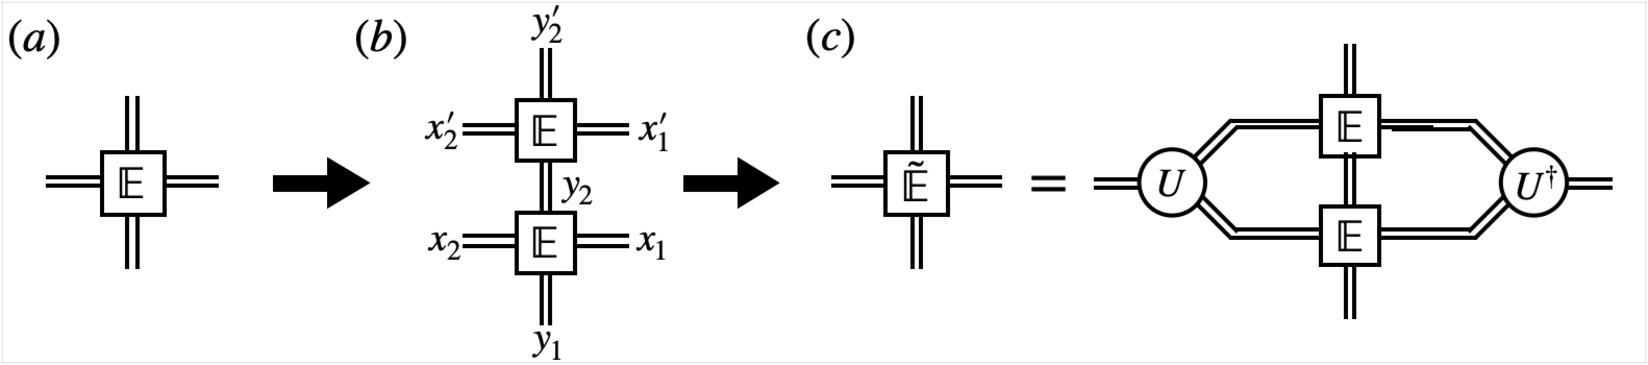
\includegraphics[width=\linewidth]{coarse_grain}
\caption{(a) Start from a one-site double tensor. (b) Merge two double tensors to form a new rank-6 tensor. (c) Apply appropriate isometries $U$ which trunctates the bond dimension}  
\label{fig:coarse_grain}
\end{figure}


Just like the standard HOTRG method, two sites are merged into a single site, generating a rank-6 tensor  $\mathbb{ E'} =  \sum_{y_2} \mathbb{ E}_{x_1,y_1,x_2,y_2}  \mathbb{ E}_{x'_1,y_2,x'_2,y'_2} $, 
where the indices of $\mathbb{ E} $ start on the right and go around clockwise to the top. 
%
This can be regarded as a rank-4 tensor by formally grouping the two indices ($x_1, x'_1$) on the right to one index, and similarly the two on the left to another. 
%
The bond dimension of tensor  $\mathbb{ E'}$  along the cylinder direction is the square of the original bond dimension of tensor $\mathbb{ E}$. 
%
Applying an appropriate isometry $U$ truncates the size of these squared bond dimensions to a fixed number, say, $D_\text{cut}$, and a truncated tensor $ \tilde { \mathbb{ E}}$ can be obtained (Fig.~\ref{fig:coarse_grain}).

To preserved the $\mathbb{Z}_2$ symmetry, we identify  $(e,e), (o,o)$ as the even sector and $(e,o),(o,e)$ as the odd sector.
%
Merging two rank-4  $\mathbb{ E} $ tensors along the $y$-axis,  we obtain a new rank-6 tensor  $\mathbb{ E'}$ which retains the $\mathbb{ Z}_2 $ structure. 
%
The $\mathbb{ Z}_2 $ symmetric isometries, $U_g (g=0,1)$ are then evaluated by performingh eigenvalue decomposition in each block of the $\mathbb{ Z}_2$  block-diagonal tensor,
\begin{align}
M_{x_1  x'_3,  x_2  x'_3} 
&=  \sum_{x_2,x_2',y_1,y_2}
\mathbb{ E'}_{x_1,x'_1,y_1,x_2,x'_2,y_1} 
\mathbb{ E'}^*_{x_2,x'_2,y_2,x_3,x'_3,y_2}.   
\end{align}
 %
Applying the isometry $U_g$  in each block generate a truncated tensor $\tilde{\mathbb{E}}$ which preserve the $\mathbb{Z}_2$ symmetry.
%
After $p$ steps of GSP-HOTRG, the final tensor represents a chain of  $2^p$ tensors that preserves the gauge symmetry.
%
The other TMs can be obtained by inserting string operator and choosing different boundary conditions. 


\subsubsection{Example: Toric Code with String Tension along $z$-Axis}
\label{subsubsec:Toric Code}
%The first model we will study is the toric code (TC) with string tension. 
To demonstrate the idea of using MES overlap to detect the phase transition, we consider the toric code (TC) model with finite string tension, which is the simplest example with the phase transition from a topological order to a topologically trivial phase~\cite{Norbert_Schuch_2013,Haegeman_2015}.
%
The string tension is added by applying the operator $Q_e(\beta_x, \beta_z) = \exp \left(  \frac{  \beta_x \sigma^x_e + \beta_z \sigma^z_e }{4}  \right)$ to the TC, 
%
\begin{align}
|\Psi(\beta_x,\beta_z)\rangle &= \prod_{e} Q_e(\beta_x,\beta_z)\times \nonumber\\
 &\prod_{v}\left(1+\prod_{e \ni v} \sigma_{e}^{x}\right) \prod_{p}\left(1+\prod_{e \in \partial p} \sigma_{e}^{z}\right) |\Omega\rangle,
\end{align}
where $e/p$ labels the the vertex/plaquette, and $ |\Omega\rangle$ indicates  the fully polarized spin state $|\Omega\rangle=\otimes_{e}|\uparrow\rangle_{e}$.
%
%At $ \beta_x =\beta_z=0$, this is the toric code ground state.  
%
For $ \beta_x =0$ and  $\beta_z \to \infty$, the system is driven to the charge condensed (CC) phase. 
%
On the other hand,  as $ \beta_x \to \infty $ and  $\beta_z $ = 0, the system is driven to the flux condensed (FC) phase.
%
 Therefore, it is expected that by tuning the parameters $ \beta_x, \beta_z$, phase transitions will occur.
%


At mentioned previously, the eigenvalues $ \lambda_{\langle a | a \rangle} =1 $, $( a =I,e,m, \epsilon )$, and zero otherwise at the $\mathbb{ Z}_2 $ topological order (TO) fixed point, indicating these four MESs are orthonormal. 
%
However, at the fixed point of the CC phase, $\lambda_{\langle I|I\rangle} = \lambda_{\langle I| e \rangle} = \lambda_{\langle  e| I \rangle} = \lambda_{\langle e | e \rangle}  = 1 $, and zero otherwise, meaning that sector $|e\rangle$ is identical to $|I\rangle$ while $|m\rangle$ and $|\epsilon\rangle$ are confined.  
%
Similarly, at the fixed point of the FC phase, we have $\lambda_{\langle I |I\rangle} = \lambda_{\langle I| m \rangle} = \lambda_{\langle   m | I \rangle} = \lambda_{\langle m | m \rangle}  = 1$. 



\begin{figure}[t]
\centering
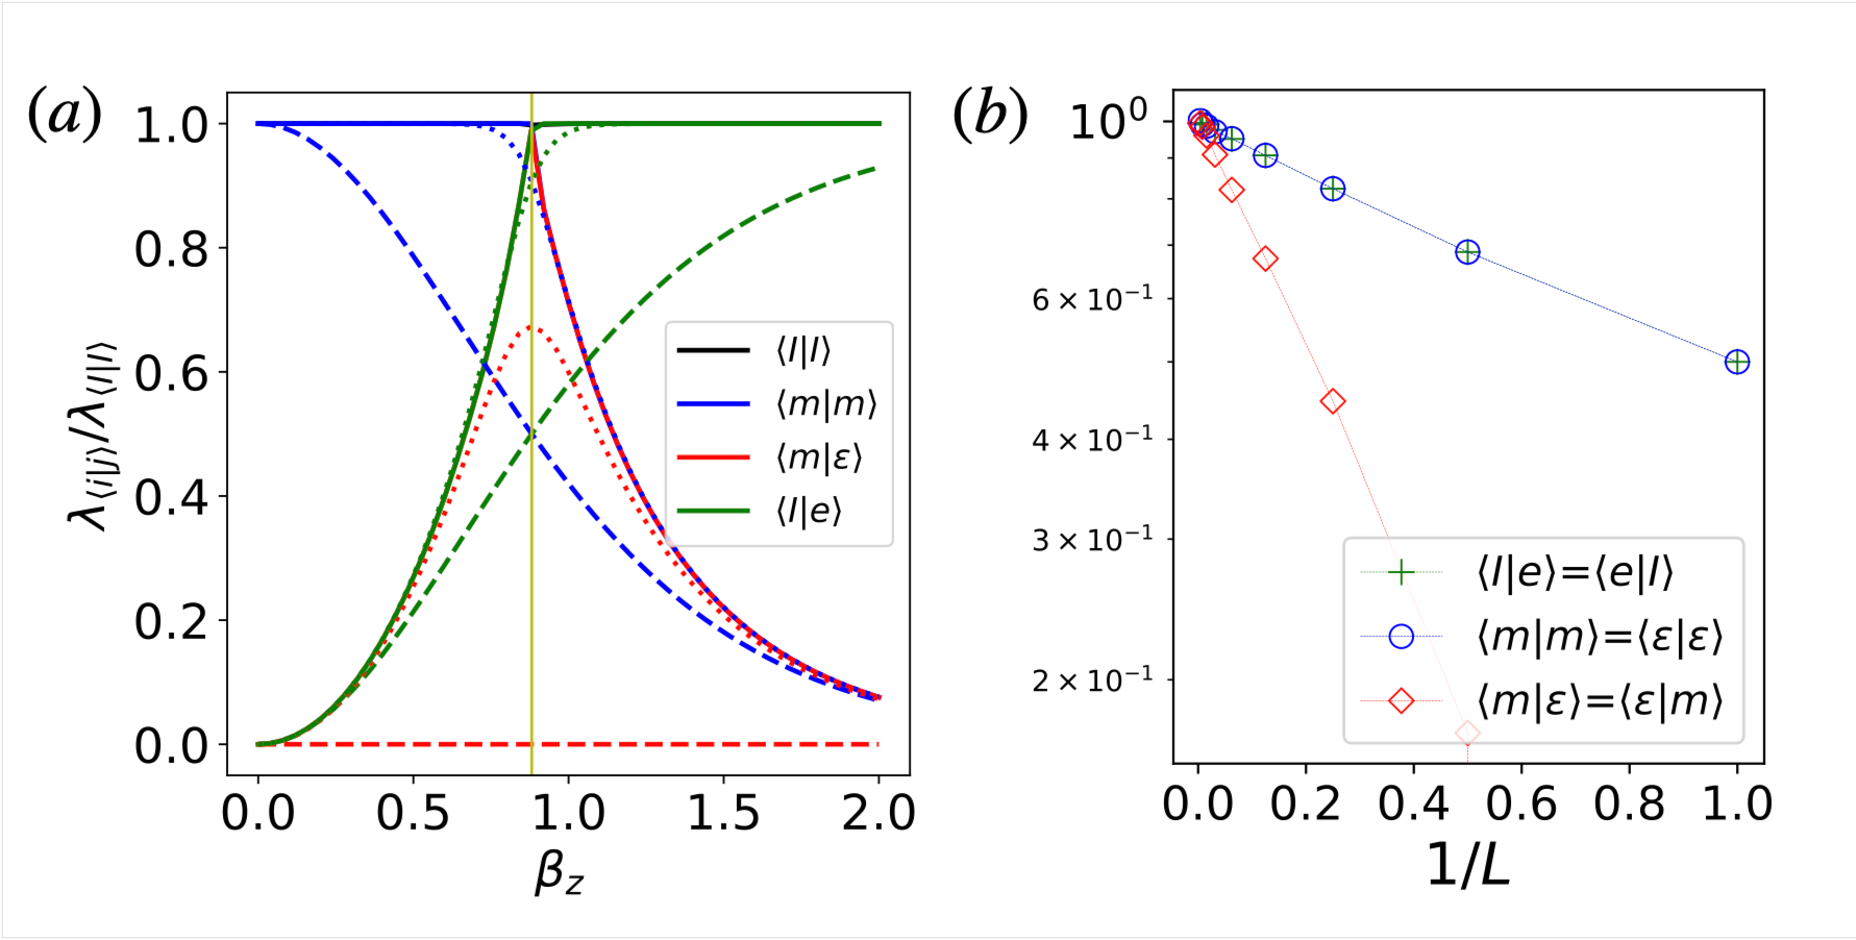
\includegraphics[width=\linewidth]{HOTRG_TC}
\caption{(a) Dominant eigenvalues  of the transfer matrices for TC with $L$ = 1 (dashed lines), $L$ = 8 (dotted lines), and $L$ = 256 (solid lines).
(b)  Dominant eigenvalues of  the  transfer matrix  for $\beta_x=0$ and $\beta_z = \beta_{z}^c$  with $D_\text{cut}=80$.
} 
\label{fig:HOTRG_TC}
\end{figure}



Along the $\beta_x=0$ axis, there exists a  phase transition from  the TO  to the CC phase as shown in Fig.~\ref{fig:HOTRG_TC}. 
%
As we increase $\beta_z$, only the regular and charge difference TMs  (red and blue blocks in Fig.~\ref{fig:tm_cylinder}(c)) are non-zero, and %we find that
there are only four distinct eigenvalues: $\lambda_{\langle I| I\rangle} = \lambda_{\langle e|e \rangle}$, $\lambda_{\langle m| m\rangle} = \lambda_{\langle \epsilon | \epsilon \rangle}$, $\lambda_{\langle I| e\rangle} =\lambda_{ \langle e| I\rangle}$,  $\lambda_{\langle m| \epsilon\rangle} =\lambda_{ \langle \epsilon| m\rangle}$.
%
We choose one in each  as a representative.
% 
The system exhibits phase transition at $\beta_z = \beta_z^c \approx 0.8814$ (Fig.~\ref{fig:HOTRG_TC}(a)).


We find  $\lambda_{\langle a | b \rangle}$ does not  have significant change for  $L > 256$; in the following, we will use $L=256$ data to represent the thermodynamic limit.  
%
For $\beta_z < \beta_z^c$, $\lambda_{\langle m|m\rangle} = \lambda_{\langle I|I\rangle} = 1$ and $\lambda_{\langle I|e\rangle} = \lambda_{\langle m|\epsilon\rangle} <1$, which is consistent with Fig.~\ref{fig:tm_cylinder}(c) that the blocks in red and blue blocks should be regarded as the same, respectively.
%
 For $\beta_z > \beta_z^c$, $\lambda_{\langle I|e\rangle} = \lambda_{\langle I|I\rangle} = 1$ and $\lambda_{\langle m|m\rangle} = \lambda_{\langle m|\epsilon\rangle} <1$. 
 %
 This indicates that the classification in Fig.~\ref{fig:tm_cylinder}(c) no longer applies; instead, we should identify the blocks in the first (fourth) column as the same.
%
At $L = 1$ and $8$, for $\beta_z < \beta_z^c$, while $\lambda_{\langle I|e\rangle} = \lambda_{\langle m|\epsilon\rangle} $ in the thermodynamic limit, $\lambda_{\langle I|e\rangle} $ is always larger than $\lambda_{\langle m|\epsilon\rangle}$. 
%
This is in fact due to the $\pi/L$ shift of momentum for $\epsilon$ mentioned before.
%
In particular, at   $\beta_z = \beta_z^c$,   $\lambda_{\langle m|m\rangle}$ and $\lambda_{\langle I|e\rangle}$ are always the same regardless of the system size, as shown in Fig.~\ref{fig:HOTRG_TC}(b). 
%
Therefore, we can accurately identify the critical point by using the crossing of $\lambda_{\langle m|m\rangle}$ and $\lambda_{\langle I|e\rangle}$ merely from a single tensor. 
%
Note that this is only true for $\beta_x = 0$. 
%
For $\beta_x\ne 0$, if we continuously deform $\beta_z$, the crossing point will shift  as we keep increasing $L$. 
%
This arises from the fact that in this scenario, not only regular and charge difference blocks but the flux and fermion difference blocks are also non-zero. 
%
However, even if we fix $\beta_x$ to other values than $0$, after $L > 4$, the crossing point is almost fixed, meaning that we can still identify the critical point using very small system sizes. 

At $L = 256$, $\lambda_{\langle I|e\rangle}  = \lambda_{\langle m|m\rangle} \rightarrow 1$. 
%
We can interpret $\lambda_{\langle I|e\rangle} \rightarrow 1$ as $|e\rangle$ begins to condense and $\lambda_{\langle m|m\rangle} \rightarrow 1$ as $|m\rangle$ begins to confine.
%
On the other hand, as mentioned previously, since no other MES can become exactly the same as $|\epsilon\rangle$, we know that $\lambda_{\langle m|\epsilon \rangle} \rightarrow 1$ indicates a gapless excitation.
%
Similarly, for the TO to FC transition, only the regular and flux difference  TMs (red and yellow blocks in Fig.~\ref{fig:tm_cylinder}(b)) are non-zero.
%
In fact, all the above observations and arguments can be directly adopted to this case once we switch the charge difference to flux difference. 


%%%%%%%%%%%

\subsection{Infinite-Plane Setting: Anyonic Excitation}
\label{subsec:infinite-plane}


Landau's symmetry breaking theory forms a paradigm to understand distinct phases of conventional matters. Once the symmetry of the Hamiltonian is given, we can construct local order parameters to characterize symmetry-breaking and symmetry-preserving states. On top of that, the universal features of the phase transition can be extracted from the order parameters' scaling behaviors near the critical points. 
%
While the MES overlap discussed Sec.~\ref{subsec:long-cylinder} can be served to qualitatively distinguish topological phases, a quantitative analysis is disallowed. Surprisingly, it turns out the order parameters for the quantitative study of topological phase transitions can be constructed through the entanglement degree of freedom within the tensor network formalism ~\citep{Haegeman_2015,2020_order_parameter}. 
%
This concept can be naturally understood by considering the fixed point of the transfer matrix in the infinite-plane setting. On the other hand, while the previous long-cylinder setting focuses on the dominant eigenvalues of the transfer matrix, TM's sub-leading eigenvalues also encode signatures about the dispersion relations of the elementary excitations \citep{2015_Zauner}. Those eigenvalues containing anyonic excitations are straightforward to apprehend numerically accessible within the infinite-plane setting. 




\subsubsection{Fixed Point: Virtual Order Parameters}
\label{subsubsec:fixed-point}
When it comes to evaluating the two-dimensional tensor network on the infinite plane, the essential task is to calculate the fixed point, i.e., the dominant eigenvector of the TM (Fig.~\ref{fig:vumps_excitation}(a)). Aside from the computational usage, the fixed point can be served as the boundary Hamiltonian of PEPS by reshaping the ket and bra layers and hence can be used to calculate the entanglement spectrum \citep{2011_entanglement}. 
%
Interestingly, owing to the $\mathbb{Z}_2$-invariant property, $\mathbb{T}$ inherits the symmetry from the tensor: $ [\mathbb{T}, Z^{\otimes \infty} \otimes \mathbb{1}^{\otimes \infty}] = [\mathbb{T},  Z^{\otimes \infty}\otimes Z^{\otimes \infty} ]  = 0$ (Fig.~\ref{fig:tm_sym}(b)), which can be derived using the pulling through condition (Fig.~\ref{fig:tm_sym}(a)). 
%
In this scheme, the fixed point may not be unique, and there are three different ``entanglement phases" \citep{2017_anyon_condensates}: 
%
(1) The fixed point is unique and respects both $ Z^{\otimes \infty}\otimes Z^{\otimes \infty} $ and $Z^{\otimes \infty} \otimes \mathbb{1}^{\otimes \infty}$ symmetry. 
%
(2) The fixed point is two-fold degenerate and respect $Z^{\otimes \infty}\otimes Z^{\otimes \infty} $ symmetry, but breaks the $Z^{\otimes \infty} \otimes \mathbb{1}^{\otimes \infty}$ symmetry. 
%
(3) The fixed point is four-fold degenerate and breaks both $ Z^{\otimes \infty}\otimes Z^{\otimes \infty} $ and $Z^{\otimes \infty} \otimes \mathbb{1}^{\otimes \infty}$ symmetry. 
%
To detect whether the fixed point respects the symmetry, one can borrow the notion of Landau's symmtry breaking paradigm by measuring the expectation value of virtual order parameters (VOPs) $ X \otimes X $ and $ X \otimes \mathbb{1} $ which anti-commutes with $ Z^{\otimes \infty}\otimes Z^{\otimes \infty} $ and $Z^{\otimes \infty} \otimes \mathbb{1}$, respectively. 
%
As discussed on Sec.~\ref{sec:Z2PEPS}, the charge anyon can be created by applying $X$ which transforms non-trivially under the group action: $ZX = -XZ$. It then follows that only $\langle X \otimes X  \rangle = 1,\langle X \otimes \mathbb{1}  \rangle = 0$ (the second case) corresponds to the topological order phase, while $\langle X \otimes X  \rangle = \langle X \otimes \mathbb{1}  \rangle = 0$ (the first case) corresponds to the charge confined phase and $\langle X \otimes X  \rangle = \langle X \otimes \mathbb{1}  \rangle = 0$ (the third case) corresponds to the charge condensed phase.
%
While in the following we only take VOPs as an alternative way to distinguish topological phases, we would like to emphasize that they can indeed be served as a quantitative study of topological phase transitions. For instance, in Ref.~\citep{2020_order_parameter}, they recover the 3D Ising critical exponents by using VOP to study the toric code model in a simultaneous $x$ and $z$ magnetic field.

\begin{figure}[h]
 \centering
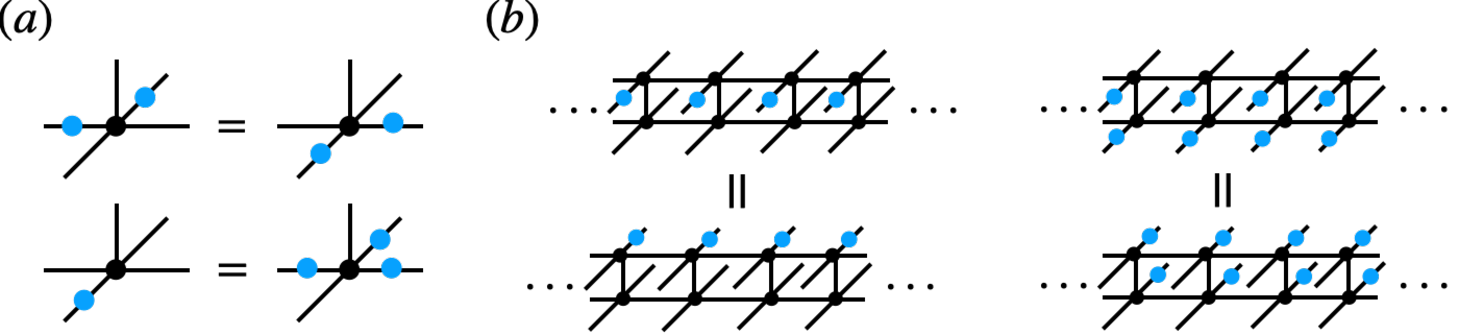
\includegraphics[width=\linewidth]{tm_sym}
\caption{(a) Pulling through condition arises from $\mathbb{Z}_2$-invariant property of the tensor. (b) Schematic representation of TM's symmetry: $[\mathbb{T}, Z^{\otimes \infty} \otimes \mathbb{1}] = [\mathbb{T}$ and  $Z^{\otimes \infty}\otimes Z^{\otimes \infty} ]  = 0$.} 
\label{fig:tm_sym}
\end{figure}

%
To evaluate VOPs, we employ variational uniform matrix product state (VUMPS) algorithm \citep{2018_vumps, 2018_faster_method, 2019_tangent_space_lecture} whose accuracy can be controlled by the bond dimension of MPS $D_{mps}$.
%
The central idea is to approximate the fixed point as a uniform MPS (Fig.~\ref{fig:vumps_excitation}(b)). The infinite-dimensional dominant eigenvalue problem is then transformed into finding the optimal MPS such that it maximizes the infinite contraction of the channel operator $T_\mathbb{E}$ (Fig.~\ref{fig:vumps_excitation}(c)), which requires the evaluation of the left(right) environment $F_L(F_R)$ by solving the left(right) dominant eigenvector the channel operator (Fig.~\ref{fig:vumps_excitation}(d)). By variationally optimizing the MPS and then updating the up and down environments, the TM fixed points can be obtained. The resulting tensors $A,F_L,$ and $F_R$ can be served as an environment for any local observable. 

\begin{figure}[h]
 \centering
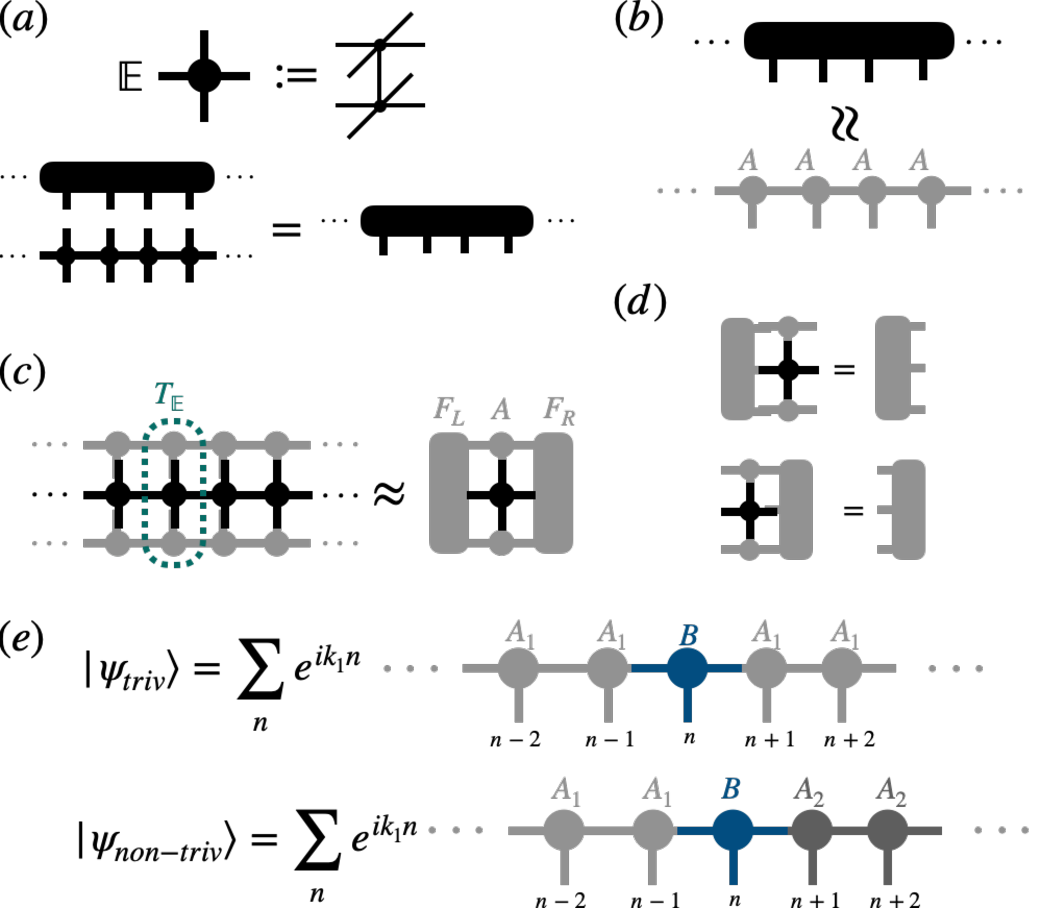
\includegraphics[width=0.8\linewidth]{vumps_excitation}
\caption{(a) The eigenequation for the transfer matrix's fixed point. Here the double tensor $W$ is obtained by contracting the physical bond of two PEPS tensors at bra and ket. (b) The translational invariant fixed point is approximated as a uniform MPS (uMPS). (c) The uMPS can be optimized by variationally maximize the channel operator $T_W$. (d) The left(right) environment is approximated by the left(right) dominant eigenvector of the channel operator. (e) The sub-dominant eigenvalues and eigenvectors can be obtained by locally perturbing one tensor and making the momentum superposition.} 
\label{fig:vumps_excitation}
\end{figure}

\subsubsection{Spectrum: Anyonic Excitations}
\label{subsubsec:tm-spectrum}
Once the fixed point of TM is obtained, the excitation spectrum can be evaluated by constructing the one-dimensional excitation ansatz ~\citep{2012_excitation}. The basic idea is to create an excitation by locally perturbing the fixed point and then make the momentum superposition to respect the translational symmetry (Fig.~\ref{fig:vumps_excitation}(d)). The perturbed tenor $B$, once being restricted to be orthogonal to the fixed point, can then be found by maximizing the overlap of the expectation value of transfer matrix: $\langle \psi(B)|\mathbb{T}|\psi(B)\rangle$. However, if the fixed point is not unique, in our case can be either 2- or 4-fold degenerate, one should also consider the topological non-trivial excitation which interpolates between two linearly independent fixed points (Fig.~\ref{fig:vumps_excitation}(d)). 

%Here come the connections with the anyonic excitation. 
For a complex TM eigenvalue $\lambda(k_1) = e^{-\epsilon(k_1) +i\phi(k_1)}$ with fixed momentum $k_1$, we can label the minus logarithm of its norm the corresponding energy $E(k_1) \sim \epsilon(k_1) = -\log{|\lambda(k_1)|}$ and assign its phase to the corresponding momentum $k_2(k_1) \sim \phi(k_1) = \arg \lambda(k_1)$. The relation between $E$ and $(k_1, k_2)$ gives the transfer matrix spectrum.
%
While overall energy scale of the local minimum of $E(k_1)$ and exact excitation energies are unknown due to the lack of Lieb-Robinson velocity \citep{1972_Lieb}, the corresponding momentum $(k_1,k_2)$ at the local minimum of $E(k_1)$ allows us to identify the location of the low-energy dispersion \cite{2015_Zauner}. 
%
If the ground state is not unique, the TM can be furthered divided into regular TM and mixed TM. It can be argued that the regular TM captures even-particle excitations, while the mixed TM describes odd-particle excitations \citep{2015_Zauner}.

\subsubsection{Example: Toric Code with String Tension along $x$-Axis}
%
To gain insights into the interpretation of TM spectrum, we revisit the typical case of TC with string tension, yet here we fix $\beta_z = 0.5$ and vary $\beta_x = 0.6,0.8,1.0,1.3$. In other words, we are studying the transition from the TO phase to the FC case. Since the TM is always hermitian, we only have the momentum label $k_1$.

For $\beta_x = 0.6,0.8$, we find that $\langle X \otimes X  \rangle = 1$ and $\langle X \otimes \mathbb{1}  \rangle = 0$, indicating the $\mathbb{Z}_2$-TO nature. 
%
The invariance of $Z^{\otimes \infty} \otimes Z^{\otimes \infty}$ action suggests that its TM eigenvector can be characterized by the eigenvalues of $ Z^{\otimes \infty} \otimes Z^{\otimes \infty} $, which can be either $+1$ (equal charge) or $-1$ (different charge).
%
Besides, owing to the symmetry breaking of $Z^{\otimes \infty} \otimes \mathbb{1}^{\otimes \infty}$, the topological non-trivial excitation of the TM, i.e., the interpolation between two degenerate fixed point, should also be considered. Overall, it follows that there are four different TM excitations. 
%
The four different classes correspond to four different kinds of TM's eigenvalues generated by the basis of minimally entangled states in the long-cylinder setting (Fig.~\ref{fig:tm_cylinder}(c)). In fact, the topological non-trivial excitations correspond to the insertion of the flux on either bra or ket, and the charge difference corresponds to the parity difference in Fig.~\ref{fig:tm_cylinder}(c).
%
Therefore, in the topological phase, one can interpret the four different classes of TM eigenvalues as vacuum excitations (trivial excitation with equal charge), charge excitations (trivial excitation with different charge, flux excitations (non-trivial excitation with equal charge), and fermion excitation (non-trivial excitation with different charge) \citep{Haegeman_2015, 2015_Zauner}. In particular, only the vacuum excitations correspond to the regular TM which describe even-particle excitations, while the other correspond to the mixed TM capturing odd-particle excitations \citep{2015_Zauner}.

\begin{figure}[h]
\centering
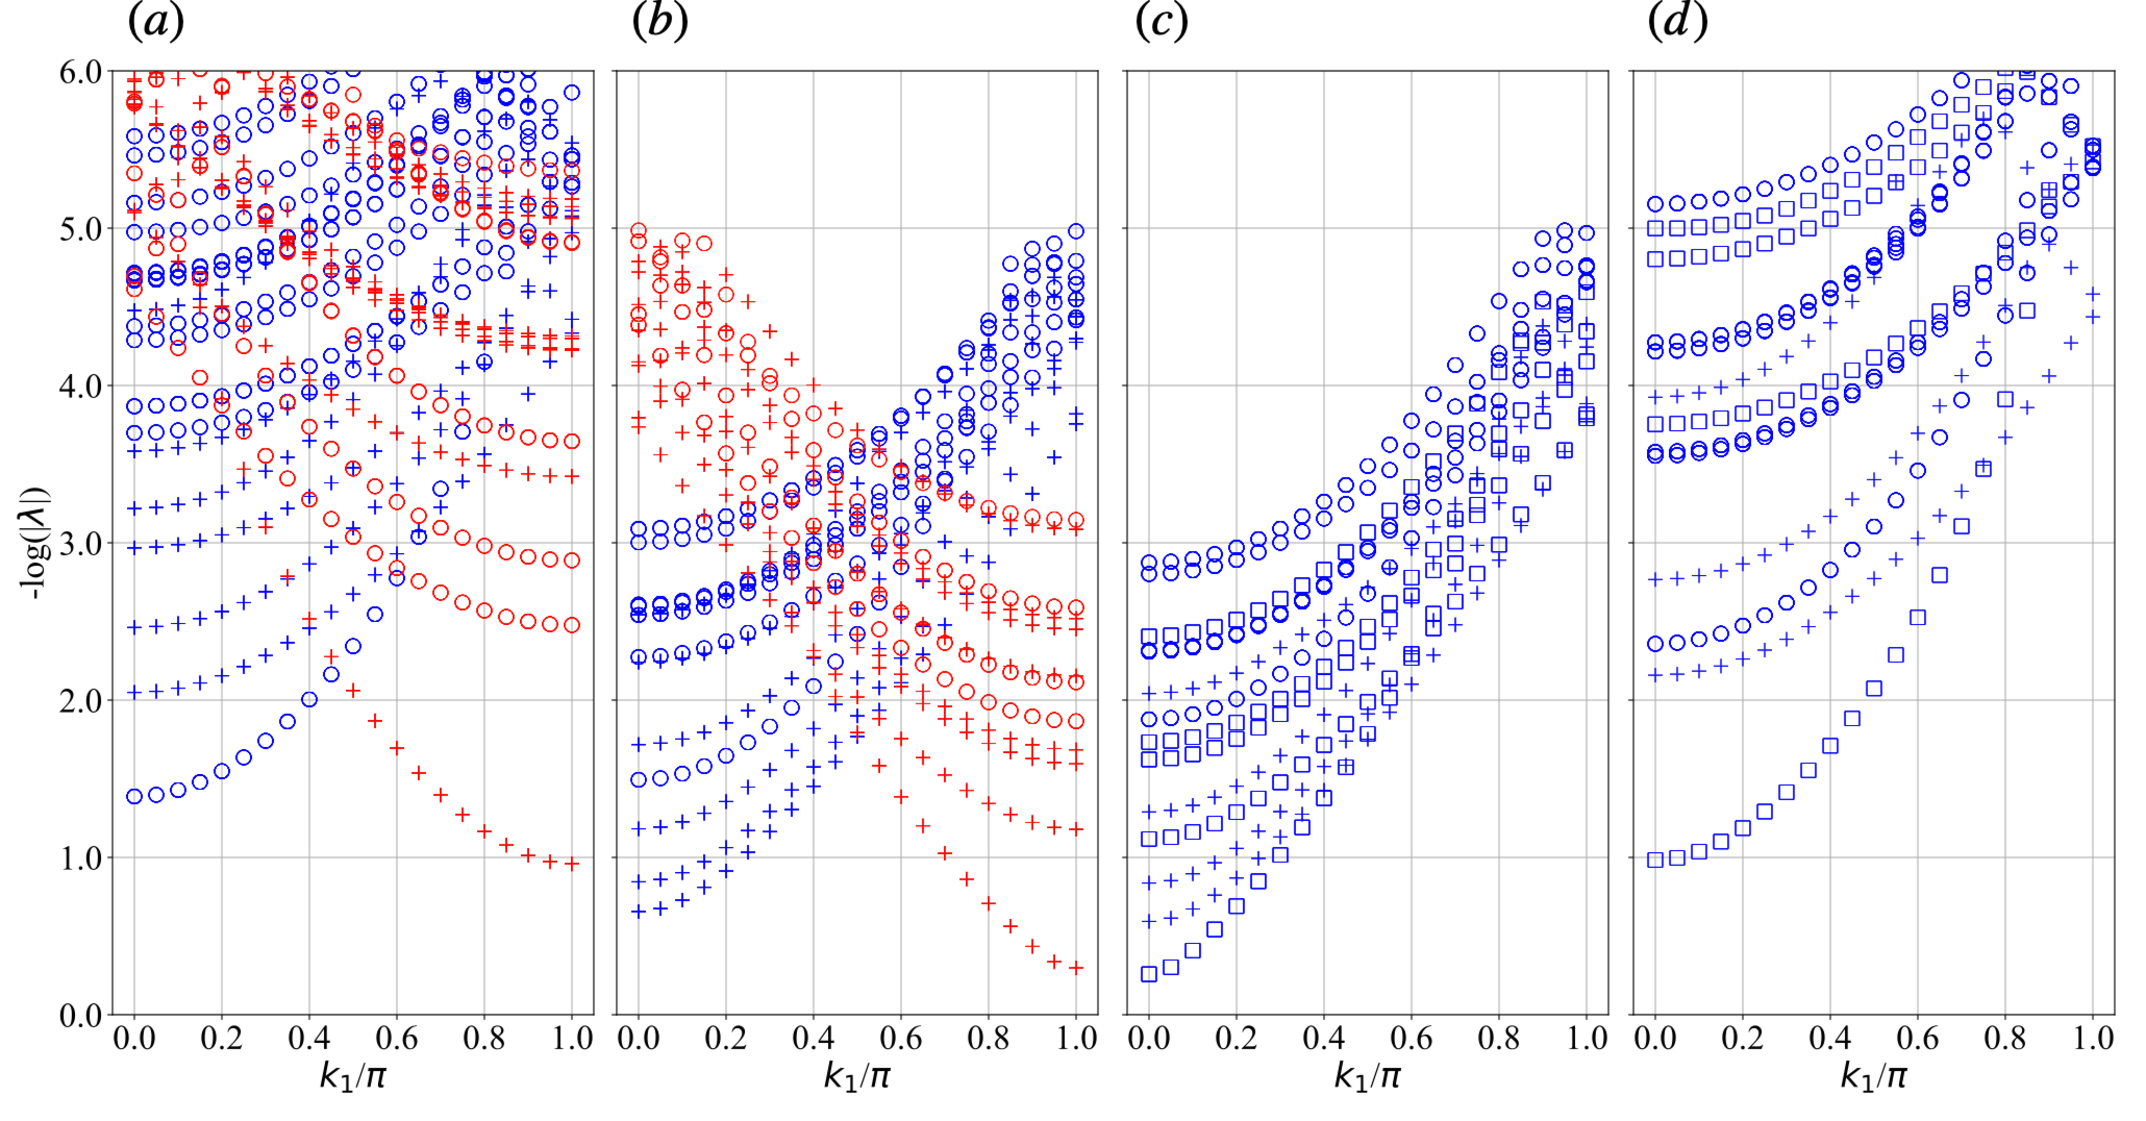
\includegraphics[width=\linewidth]{spectrum_TC}
\caption{Transfer matrix spectrum for the toric code with string tension $\beta_z = 0.5$ and $\beta_x = 0.6$ (a), $0.8$ (b), $1.0$ (c), $1.3$ (d).} 
\label{fig:spectrum_TC}
\end{figure}
%
Fig.~\ref{fig:spectrum_TC}(a)(b) show the TM spectrum for $\beta_x = 0.6$ and $0.8$. Here we follow the labels in Ref.~\citep{Haegeman_2015} to denote the equal(different) charge as plus(circle) signs while the topological trivial(non-trival) excitations as blue(red) colors. As $\beta_x$ increase from $0.6$ to $0.8$, one can observe that the gap in the flux sector decreases, indicating the flux begin to condense.
%

As we further increase $\beta_x$ to $1.0$, we found that  $\langle X \otimes X  \rangle = \langle X \otimes \mathbb{1}  \rangle = 0$, indicating the system are driven into the charge confined (also the flux condensed) phase. In this circumstance, the uniqueness of the fixed point indicates that there is no domain wall excitations. On the other hand, the charge number in the individual bra and ket layer can now be measured owing to the  extra $Z^{\otimes \infty} \otimes \mathbb{1}^{\otimes \infty}$ symmetry comparing to the TO phase. 
%
In terms of the 16 blocks of TMs defined within the long-cylinder setting, this implies that the classification in Fig.~\ref{fig:tm_cylinder}(c) no longer applies; instead, we should identify the blocks in the first(fourth) row as the same class. 
%
Fig.~\ref{fig:spectrum_TC}(c)(d) show the TM spectrum for $\beta_x = 1.0$ and $1.3$. One can observe that the topological non-trivial excitations (red color) disappear; instead, a new class of excitations characterized by the the odd charge number on both bra and ket (sqaure in Fig.~\ref{fig:spectrum_TC}(c)(d)) emerges. The gap in the new sector indicates that a single charge excitations can no longer exist can must be confined with other charge anyon.

Similarly, for the TO to CC transitions, we will find that the expectation value  $\langle X \otimes \mathbb{1}  \rangle$ switch from $0$ to $1$. In this case, the fixed point is 4-fold degenerate and there will be two kinds of domain wall excitations. The breaking of both $Z^{\otimes \infty} \otimes \mathbb{1}^{\otimes \infty}$ symmetry indicates that there is no charge can be measured anymore.

\chapter{Kitaev Model and Tensor Network Study}

In this chapter, we will use 
\section{Spin-$1$ Honeycomb Kitaev Model}

Hamiltonian of Kitaev honeycomb model is defined as 
\begin{equation}
H = -J_x \sum_{ \langle i,j  \rangle_x } S_i^xS_j^x - J_y \sum_{\langle i,j \rangle_y} S_i^yS_j^y  - J_z\sum_{\langle i,j \rangle_z} S_i^zS_j^z,
\end{equation}
where $\langle i,j \rangle_\gamma$ represents the nearest neighboring sites connecting through $\gamma$-links where $\gamma = x,y,z$ (Fig.~\ref{fig:honeycomb_LG}(a)). To gain some insights into the model, one can consider the strong anisotropic limit: $J_x = 1, J_y = J_z = 0$. In this scenario, the ground states degeneracy is exponentially large with the system size, and its basis can be characterized by the effective spin $|\uparrow \rangle =  |x,+\rangle |x, + \rangle$ and $|\downarrow \rangle = |x,-\rangle |x, -\rangle$ defined on each $x$-link, which acquires the lowest energy  $-\langle \uparrow ( \downarrow)| S_i^xS_j^x| \uparrow  (\downarrow) \rangle$. Here $|x,\pm \rangle$ is the eigenstate of $S^x$ with eigenvalues $\pm S$. In a hand-waving perspective, the Kitaev Hamiltonian can be understood as a mechanism describing three different kinds of interaction generating by $J_x,J_y,J_z$.

Another important property of the model is that it has a constant of motion: $W_p = U_1^xU_2^yU_3^z U_4^xU_5^yU_6^z$ ($U^\gamma = e^{i\pi S^\gamma}$), the flux operator, which commutes with the Hamiltonian (Fig.~\ref{fig:honeycomb_LG}(a)). Here $p$ denotes the site label of the hexagonal plaquettes. One can then sectorize the Hilbert space using the eigenvalues $w_p$ for the flux operator. For spin 1, it has been numerically shown that the ground state lives in the vortex-free sector $w_p = +1$ \citep{spin_one_half, lee2020anisotropy}.

\begin{figure}[h]
\centering
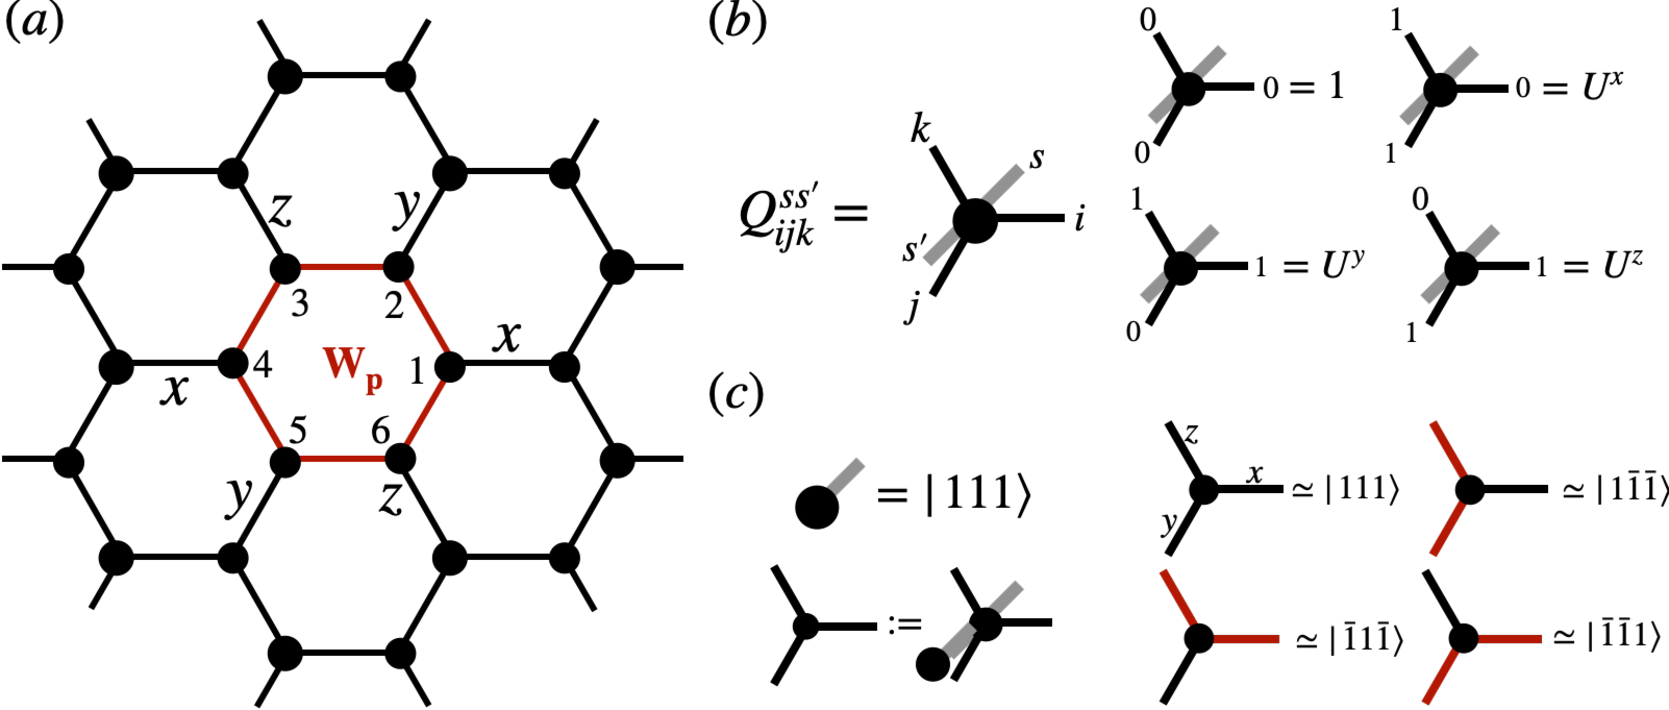
\includegraphics[width=\linewidth]{honeycomb_LG}
\caption{(a) Honeycomb lattice and the flux operator. (b) Definition of the LG tensor. (c) The resulting state of LG tensor acting on the initial product state $|111\rangle$ (up to a phase factor). Here we dentoe $1$ has string (red color) and $0$ as no string (black color).} 
\label{fig:honeycomb_LG}
\end{figure}

\subsection{Loop Gas Operator and Loop Gas States}
To obtain the LG states, let us first consider an LG operator
 $\hat{Q}_{\text{LG}} = \text{tTr}\prod_\alpha {Q}^{ss'}_{i_\alpha j_\alpha k_\alpha}|s\rangle \langle s'| $ with the LG tensor defined as
\begin{equation}
Q_{000} = \mathbb{1}, Q_{011} = U^x, Q_{101} = U^y, Q_{110} = U^z.
\end{equation}
where $U^\gamma = e^{i \pi S^\gamma}$ is the $\pi$-rotation operator for a given spin (Fig.~\ref{fig:honeycomb_LG}(b)) ~\cite{lee2020anisotropy}. One of the important properties of LG tensor is that the $\pi$-rotation operator $U^\gamma$ acting on the physical Hilbert space can be transformed into two $\sigma^x$ actions on the virtual space (Fig.~\ref{fig:LG_property}(a)). This property  guarantees that $\hat{Q}_{\text{LG}}$ is a projector to the vortex-free space: $\hat{W}_p\hat{Q}_{\text{LG}} = \hat{Q}_{\text{LG}}\hat{W}_p = \hat{Q}_{\text{LG}}$ (Fig.~\ref{fig:LG_property}(b)). 
Another useful feature of LG tensor is that it is invariant under the global $ \mathbb{Z}_2$ symmetry on the virtual dimensions: $Q(u_g \otimes u_g \otimes u_g) = Q $ with $u_g = \mathbb{1}_2, {\sigma}^z$ (Fig.~\ref{fig:LG_property}(c)), making any tensor applied by $\hat{Q}_{\text{LG}}$ also enjoys the global $\mathbb{Z}_2$ symmetry with $u_g = \mathbb{1}_2 \otimes \mathbb{1}_{D_0}, {\sigma}^z \otimes \mathbb{1}_{D_0}$, where $D_0$ is the bond dimension of the original tensor. 
%
As discussed in Sec.~\ref{sec:Z2PEPS}, this $\mathbb{Z}_2$-invariant property allows a construction of flux (a string of $\sigma^z$ acting on virtual dimensions) and charge (a pair of $\sigma^x$ acting on virtual dimensions) based on the notion of parent Hamiltonian. Furthermore, owing to the property in Fig.~\ref{fig:LG_property}(a), the creation of flux anyon pair also correspond to two vortices $w_p = -1$ at the end point of the string $(\sigma^z)^{\otimes L}$ (Fig.~\ref{fig:LG_property}(d)).

\begin{figure}[h]
 \centering
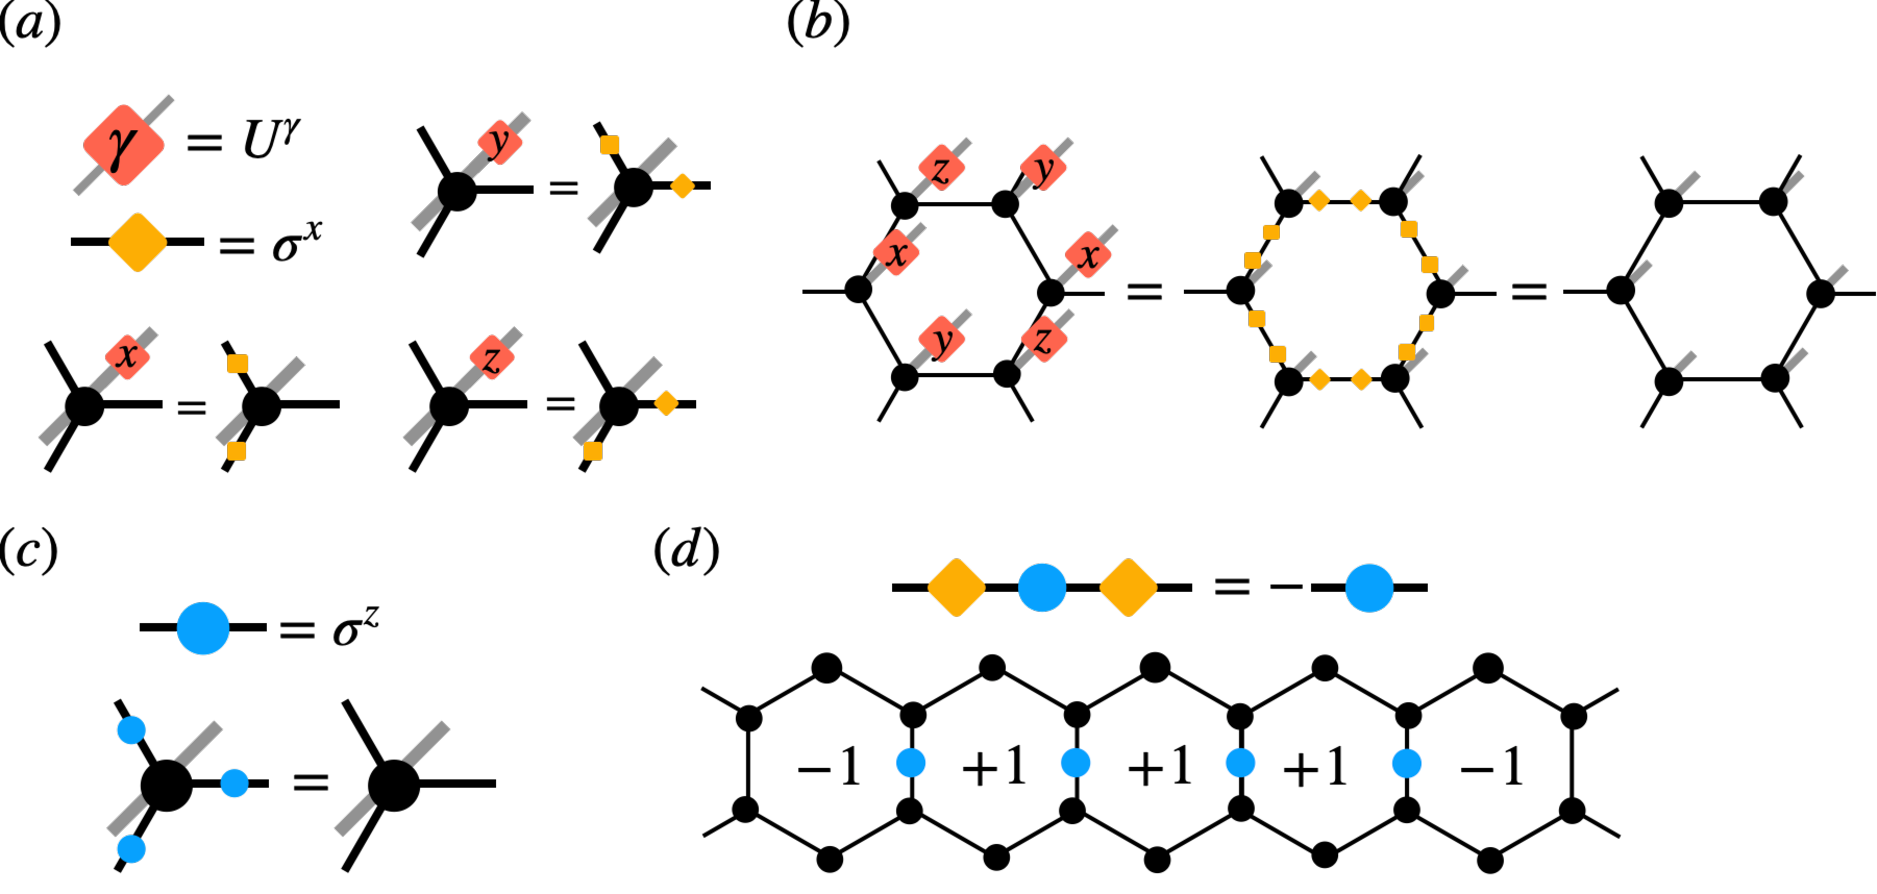
\includegraphics[width=\linewidth]{LG_property}
\caption{(a) The $\pi$-rotation operator $U^\gamma$ acting on the physical Hilbert space can be transformed into two $\sigma^x$ actions on the virtual space. (b) Using the property in (a), one can show that $\hat{Q}_{\text{LG}}$ is a projector to the vortex-free space. (c) LG tenosr is $\mathbb{Z}_2$-invariant. (d) A string  $(\sigma^z)^{\otimes L}$ acting on the virtual dimension corresponds to creating two vorticed at the end point of the string.} 
\label{fig:LG_property}
\end{figure}

The LG state can then be obtained by applying $\hat{Q}_{\text{LG}}$ on one of the classical ground states $|\psi \rangle = \otimes_\alpha |111\rangle_\alpha$, where $|111\rangle$ is defined by $\langle 111| S^\gamma |111\rangle = (S,S,S)/\sqrt{3}$. Using the property that the non-trivial action of $\hat{Q}_{\text{LG}}$ is the $\pi$-rotation operator, one can derive the resulting state of LG tensor acting on the initial product state Fig.~\ref{fig:honeycomb_LG}(c). The $\pi$-rotation feature guarantees that if the initial state is the classical ground states, all the resulting states after applying $\hat{Q}_{\text{LG}}$ are also the classical ground states. For instance, the states of site 2 and site 3 connecting through $x$-link in Fig.~\ref{fig:honeycomb_LG} are $|\bar{1}\bar{1}1 \rangle$ and $|\bar{1}1\bar{1}\rangle$, respectively. Since their signs of the $x$-component are flipped simultaneously, the $x$-bond's energy is unchanged comparing with the initial states $\otimes_\alpha|111\rangle$. Therefore, one can understand the LG states as an equal weight superposition of all the looped classical ground states: $| \psi_{\text{LG}} \rangle = \sum | \text{all looped classical ground states} \rangle$. From this perspective, the energy of LG states should be exact in the high-spin limit, which can be verified by numerical study comparing with the classical energy $E = -1/2S^2N$ \citep{Baskaran_2008}:

\begin{center}
 \begin{tabular}{||c |c| c|| c |c| c||} 
 \hline
S & Energy & Energy/$S^2$ & S & Energy & Energy/$S^2$   \\ 
 \hline
 1/2 & -0.1635 & -0.654 & 2 & -2.000 & -0.5 \\ 
\hline
 1 & -0.5056 & -0.5056 & 5/2 & -3.125 & -0.5 \\ 
 \hline
 3/2 & -1.1255 & -0.5002 & 3 & -4.500 & -0.5 \\ 
 \hline
\end{tabular}
\end{center}

%To evaluate the observable in the infinite 2D tensor network, we employ varitaional uniform MPS (VUMPS) algorithm \citep{2018_vumps, 2018_faster_method, 2019_tangent_space_lecture} whose accuracy can be controlled by the bond dimension $D_{mps}$.
The evaluation of the energy can be done by using VUMPS, as discussed in Sec~\ref{subsec:infinite-plane}. From the table, one can observe that the energy for spin one-half and spin one shows deviation. This lies from the fact that when spin $S$ is small, the basis of LG state $|111\rangle , |1\bar{1}\bar{1}\rangle ,|\bar{1}1\bar{1}\rangle  |\bar{1}\bar{1}1\rangle ,$  are not orthogonal to one another. As spin goes up, the overlap between those states goes to zero exponentially: ${\ |\langle 111|1\bar{1}\bar{1}\rangle| =  \big (\frac{1}{3} \big)^{S} }$. Following the same logic, one can also obtain another orthogonal LG states by applying $\hat{Q}_{\text{LG}}$ on the initial product states $|\psi \rangle = \otimes_\alpha |\bar{1}\bar{1}\bar{1}\rangle_\alpha$.

\subsection{Imaginary Time Evolution}
While LG states capture some essential features of the spin-1 Kitaev model, its energy is much more higher than the energy obtained from exact diagonalization \citep{2018_exact_spin1}. To obtain the ground state, one can either construct higher-order vatiational ansatz or do the imaginary time evolution (ITE) (Fig.~\ref{fig:ITE_energy}(a) \cite{simple-update}. However, both of them have some limitations. While the higher-order ansatz preserve both the $\mathbb{Z}_2$-invariant property and vortex-free condition, its efficiency of lowering the energy is worse than ITE. 
%
On the other hand, while keeping the degenerate eigenvalues during the singular value decomposition for ITE, the wave functions will remain the vortex-free \citep{2020-spin-one-kitaev}, the $\mathbb{Z}_2$-invariant property is no longer guaranteed.


To obtain reliable PEPS ground states and strictly enforce both vortex-free and $\mathbb{Z}_2$-invariant property, we modify the construction by first doing the ITE on the initial product state, and then apply the LG projector. Nonetheless, applying the LG projector will double the bond dimension, and one should make sure that resulting state $Q_{\text{LG}}e^{-\tau H}|\psi_0 \rangle$ should have lower energy than purely doing the ITE $e^{-\tau H}|\psi_0 \rangle$ for the same bond dimension. From Fig.~\ref{fig:ITE_energy}(b), one can observe that the for small total bond dimension $D$, purely applying ITE yields lower energy. As the bond dimension increases, $Q_{\text{LG}}e^{-\tau H}|\psi_0 \rangle$ outweigh $e^{-\tau H}|\psi_0 \rangle$. Since the two-site operator $e^{-\tau S_i^\gamma S_j^\gamma}$ applied during the ITE commutes with the LG projector: $[e^{-\tau S_i^\gamma S_j^\gamma}, Q_{\text{LG}}] = 0$, one can also numerically show that $Q_{\text{LG}}e^{-\tau H}|\psi_0 \rangle$ acquire the same energy as $e^{-\tau H}|\psi_\text{LG} \rangle = e^{-\tau H}Q_{\text{LG}}|\psi_0 \rangle$.

\begin{figure}[h]
 \centering
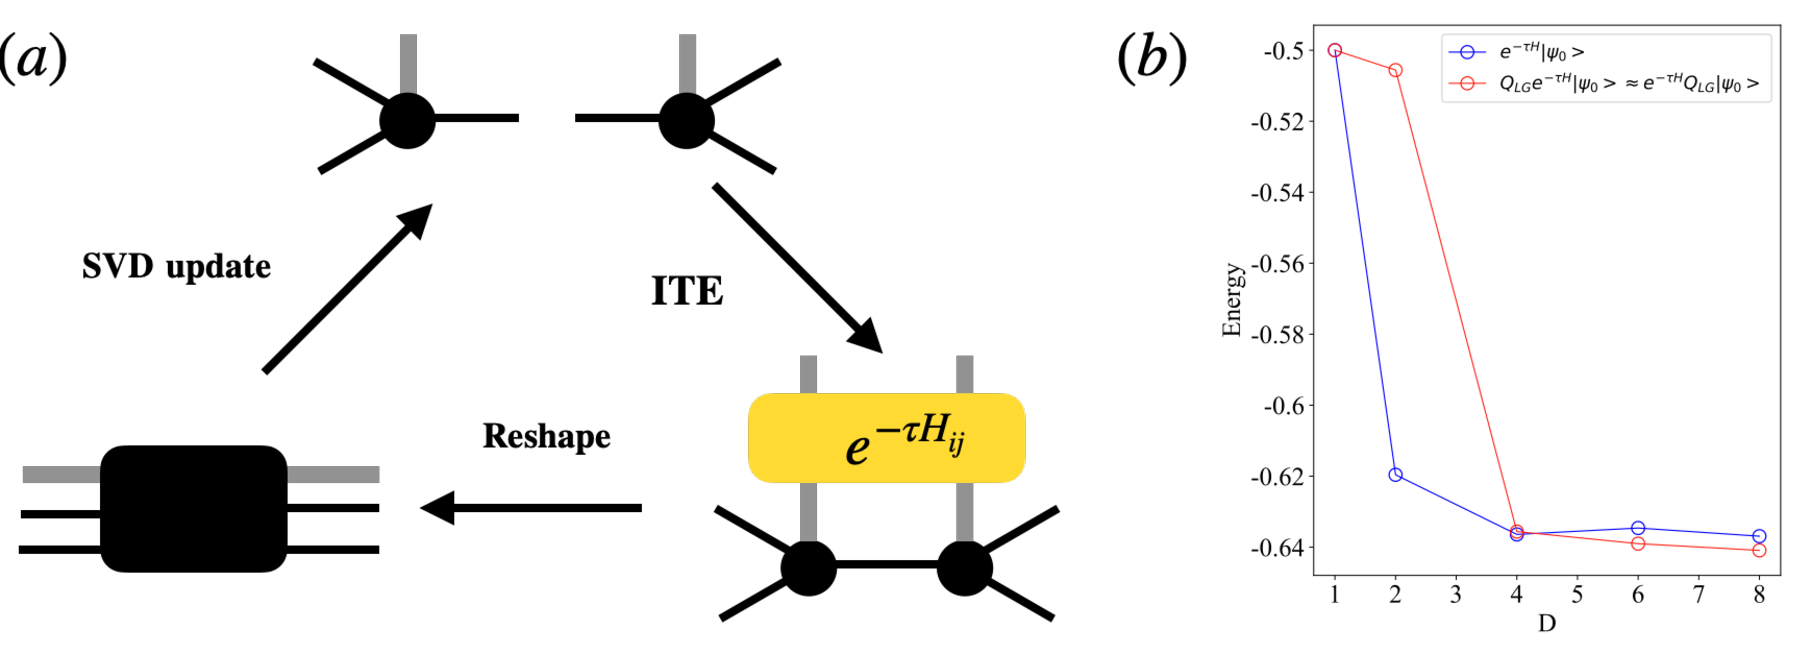
\includegraphics[width=\linewidth]{ITE_energy}
\caption{(a) Schematic implementation of the simple update. (b) Comparison of energy between $Q_{\text{LG}}e^{-\tau H}|\psi_0 \rangle$ and $e^{-\tau H}|\psi_0 \rangle$ for the same bond dimension.}
\label{fig:ITE_energy}
\end{figure}

\subsection{Transfer Matrix Spectrum}
Throughout the calculation, we find that the $\langle X \otimes X \rangle = 1$ and $\langle X \otimes \mathbb{I} \rangle = 0$ regardless of the bond dimension, suggesting that the ground state of spin-1 Kitaev model lies in the $\mathbb{Z}_2$ spin liquid phase as elaborated in Sec.~\ref{subsec:infinite-plane}.

\begin{figure}[h]
 \centering
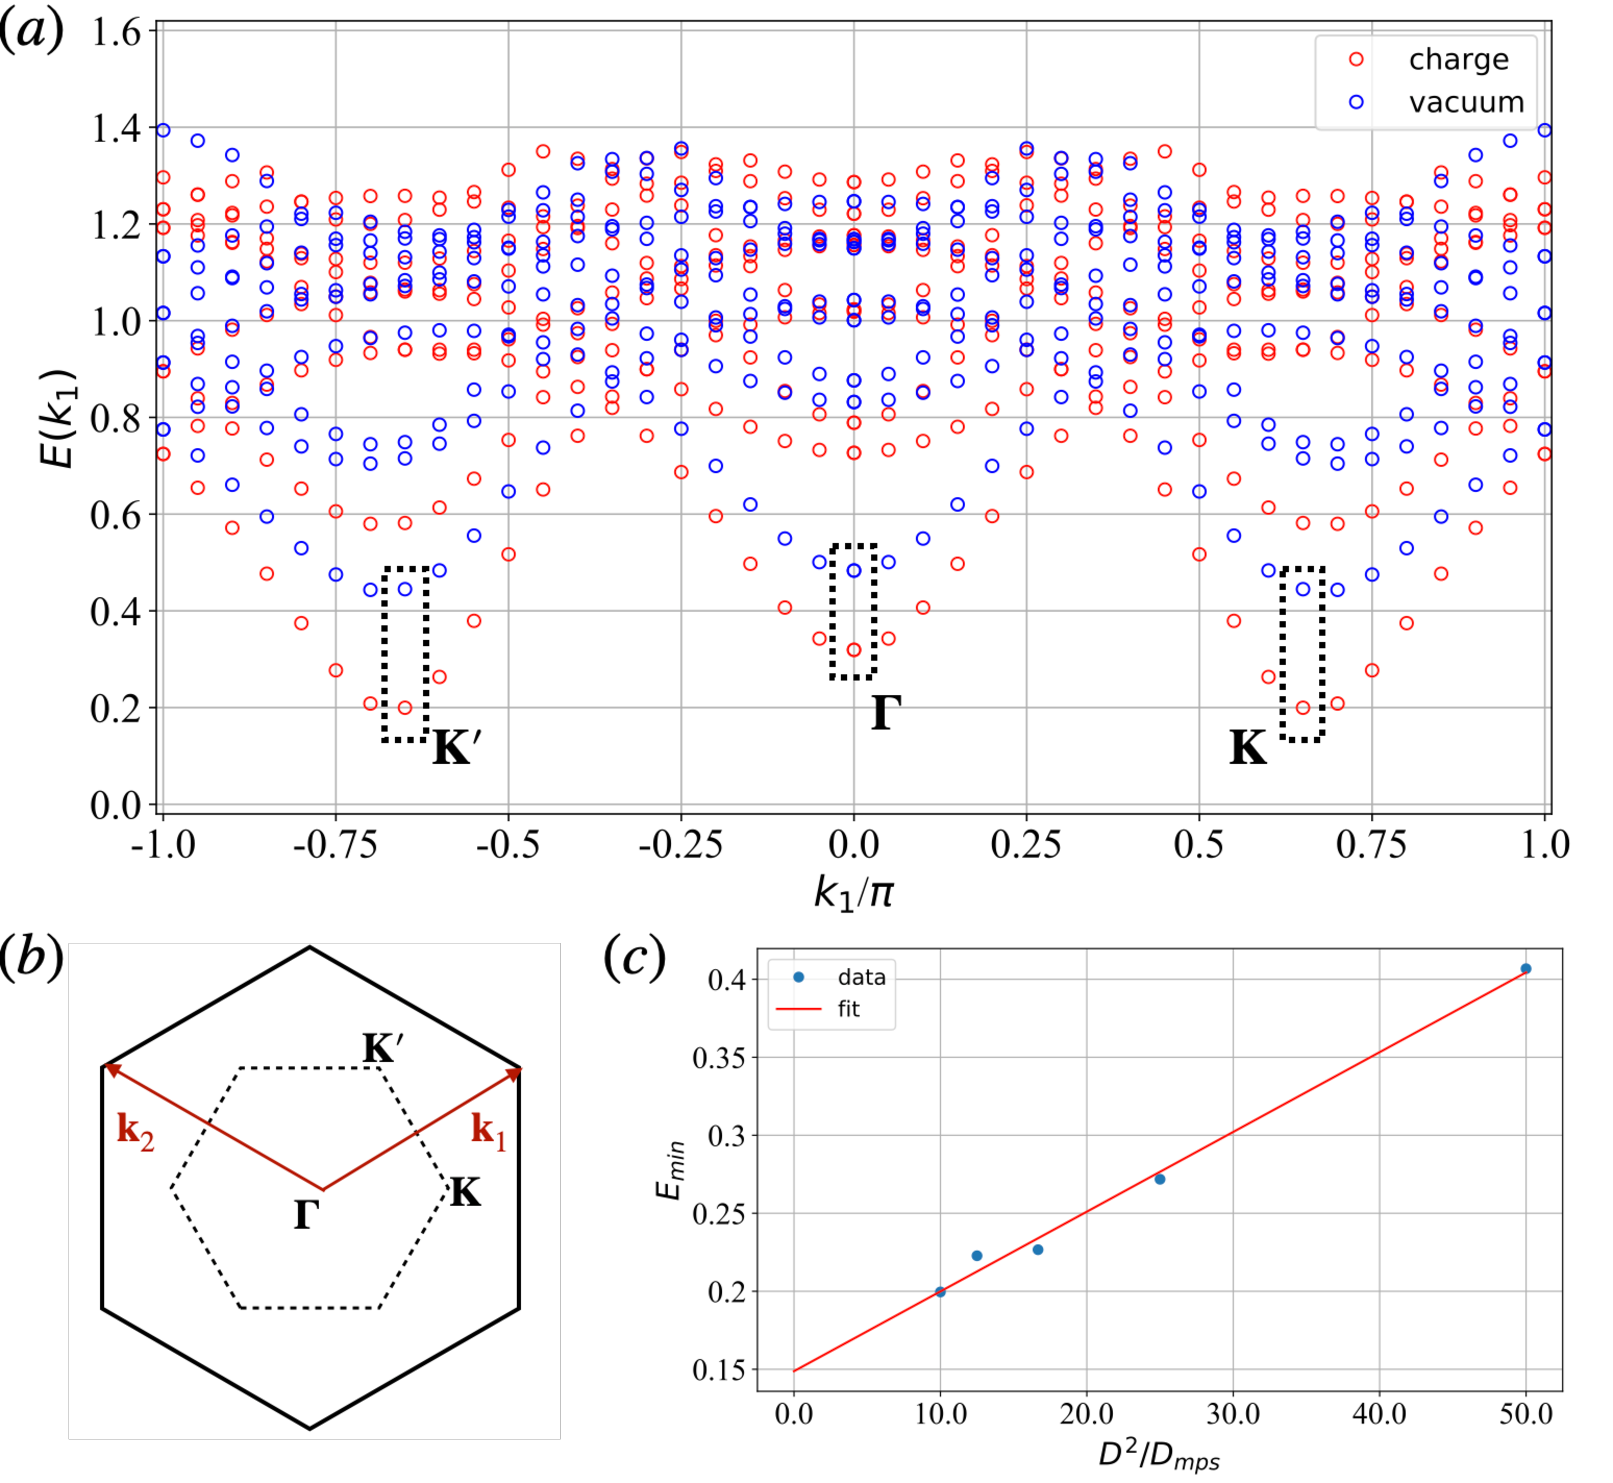
\includegraphics[width=\linewidth]{D10spect_BZ_extrapolate}
\caption{(a) Transfer matrix spectrum for the PEPS tensor with $(D,D_\textbf{mps}) = (10, 10)$. (b) Brillouin zone with labeled positions of the minimum of TM spectrum. (c) The smallest excitation energy of the $D = 10$ PEPS wavefunction as a function of $D_\text{mps}$.} 
\label{fig:D10spect_BZ_extrapolate}
\end{figure}

Using the correspondence $E(k_1) \sim \epsilon(k_1) = -\log{|\lambda(k_1)|}$ for TM's complex eigenvalue $\lambda(k_1) = e^{-\epsilon(k_1) +i\phi(k_1)}$ and the excitation energy $E(k_1)$ \citep{2015_Zauner}, the TM spectrum for PEPS states with bond dimension $D=10$ are shown in Fig.~\ref{fig:D10spect_BZ_extrapolate}(a).
%
Minima of both the charge and vacuum excitations are clearly identified at $k_1 = 0, 2\pi/3,$ and $-2\pi/3$.
%
To gain more insights into the two-dimensional system, we consider the momentum in $y$-direction, which can be acquired from the phase of the complex eigenvalues $k_2(k_1) \sim \phi(k_1) = \arg \lambda(k_1)$  \citep{2015_Zauner}. 
%
The location of three minimum excitations are then identified at $(k_1,k_2) = (0,0), (2\pi/3, -2\pi/3),$ and $(-2\pi/3, 2\pi/3)$, suggesting that the spin-$1$ Kitaev model harbors three low-lying charge excitations at  $\boldsymbol{\Gamma}, \bold{K},$ and $\bold{K'}$ symmetric points in the Brillouin zone (Fig.~\ref{fig:D10spect_BZ_extrapolate}(b)).
%

On the other hand, since the global minima lies at $\bold{K} (\bold{K'})$: $\epsilon_\textbf{min} = \epsilon(\bold{K}) = \epsilon(\bold{K'}) <  \epsilon(\boldsymbol{ \Gamma})$, the low-lying vacuum excitations at  $\boldsymbol{\Gamma}, \bold{K},$ and $\bold{K'}$ are attributed to the two-particle charge excitations $\epsilon(\bold{K}) + \epsilon(\bold{K'})$, $\epsilon(\bold{K'}) + \epsilon(\bold{K'})$, and $\epsilon(\bold{K}) + \epsilon(\bold{K})$, respectively.

To estimate the system's gap, we calculate the lowest TM spectrum energy as a function of the accuracy-contolled dimension $D_{mps}$ (Fig.~\ref{fig:D10spect_BZ_extrapolate}(c)). Naive extrapolation puts an upper bound $\epsilon = 0.149J$ on the excitation gap. However, the possibility of a gapless spin liquid in the infinite bond dimension (both $D$ and $D_{mps}$) cannot be completely ruled out.  
\section{Spin-$1/2$ Star Lattice Kitaev Model}
\label{sec:star_lattice}

We extend the ideas developed in Sec.~\ref{subsec:long-cylinder} to study the phase transition from an Abelian to a non-Abelian  spin TO.
%
We will study the quantum phase transition of the Kitaev model on the star lattice by studying TMs built from  the $\mathbb{Z}_2$-injective  LG and SG states~\cite{spin_one_half,2020-spin-one-kitaev,lee2020anisotropy}.
%
The Hamiltonian is defined as~\cite{Hong_Ya_2007}
\begin{equation}
H = -J\sum_{{\langle i,j \rangle}_\gamma} S^\gamma_iS^\gamma_j - J'\sum_{\langle ij\rangle \in \gamma'}S^{\gamma'}_i S^{\gamma'}_j
\label{eq:starKitaev}
\end{equation}
where ${\langle i,j \rangle}_\gamma$  and ${\langle i,j \rangle}_\gamma'$  are 
the pairs on  the intratriangle  ($\gamma = x,y,z$) and  the intertriangle  ($\gamma'=x',y',z'$) links connecting site $i $ ans $j$ as shown in Fig.\ref{fig:star_lattice}(a), respectively.  
%
The Hamiltonian can be block diagonalized by the eigenvalues of two types of flux operators defined on the triangle plaquette $\hat{V}_p = \hat{\sigma}_1^z\hat{\sigma}_2^x\hat{\sigma}^y_3$ and the dodecagon plaquete $\hat{W}_p = \hat{\sigma}_1^x\hat{\sigma}_2^z\hat{\sigma}^y_3...\hat{\sigma}_{12}^y$, where $\hat{\sigma}^i, i = x,y,z$ is the Pauli matrix.
%
To gain insights into the model, we  consider two extreme limits: the isolated-dimer limit ($J =0,J'=1$) and the isolated-triangle limit ($J =1,J'=0$) [Fig.\ref{fig:star_lattice}(b)].
%
The perturbative study in Ref.~\cite{KSL_perturbative} shows that in the isolated-dimer limit, while the Hamiltonian does not map exactly onto the standard toric code, the ground state is the same as the toric code on the honeycomb lattice. 
%
On the other hand, the isolated-triangle limit can be mapped onto the Kitaev honeycomb model at the isotropic point which exhibits a non-Abelian topological order. 
%
This suggests that there should exist a phase transition between the two phases. 
%
Exact results shows that the model has two distinct gapped phases: $\mathbb{Z}_2$ topological order when $J'/J >\sqrt{3}$ and non-Abelian CSL with Ising anyon, when   $J'/J <\sqrt{3}$. The latter can be distinguished from the former by its three-fold topological degeneracies which can be labeled using MES basis in Ising anyon: $|I\rangle, |\sigma\rangle, |\epsilon\rangle$.
%
In both regime, the ground states live in the vortex-free sector $\{W_p = 1, V_p = 1\}$.
%

\begin{figure}[t]
\centering
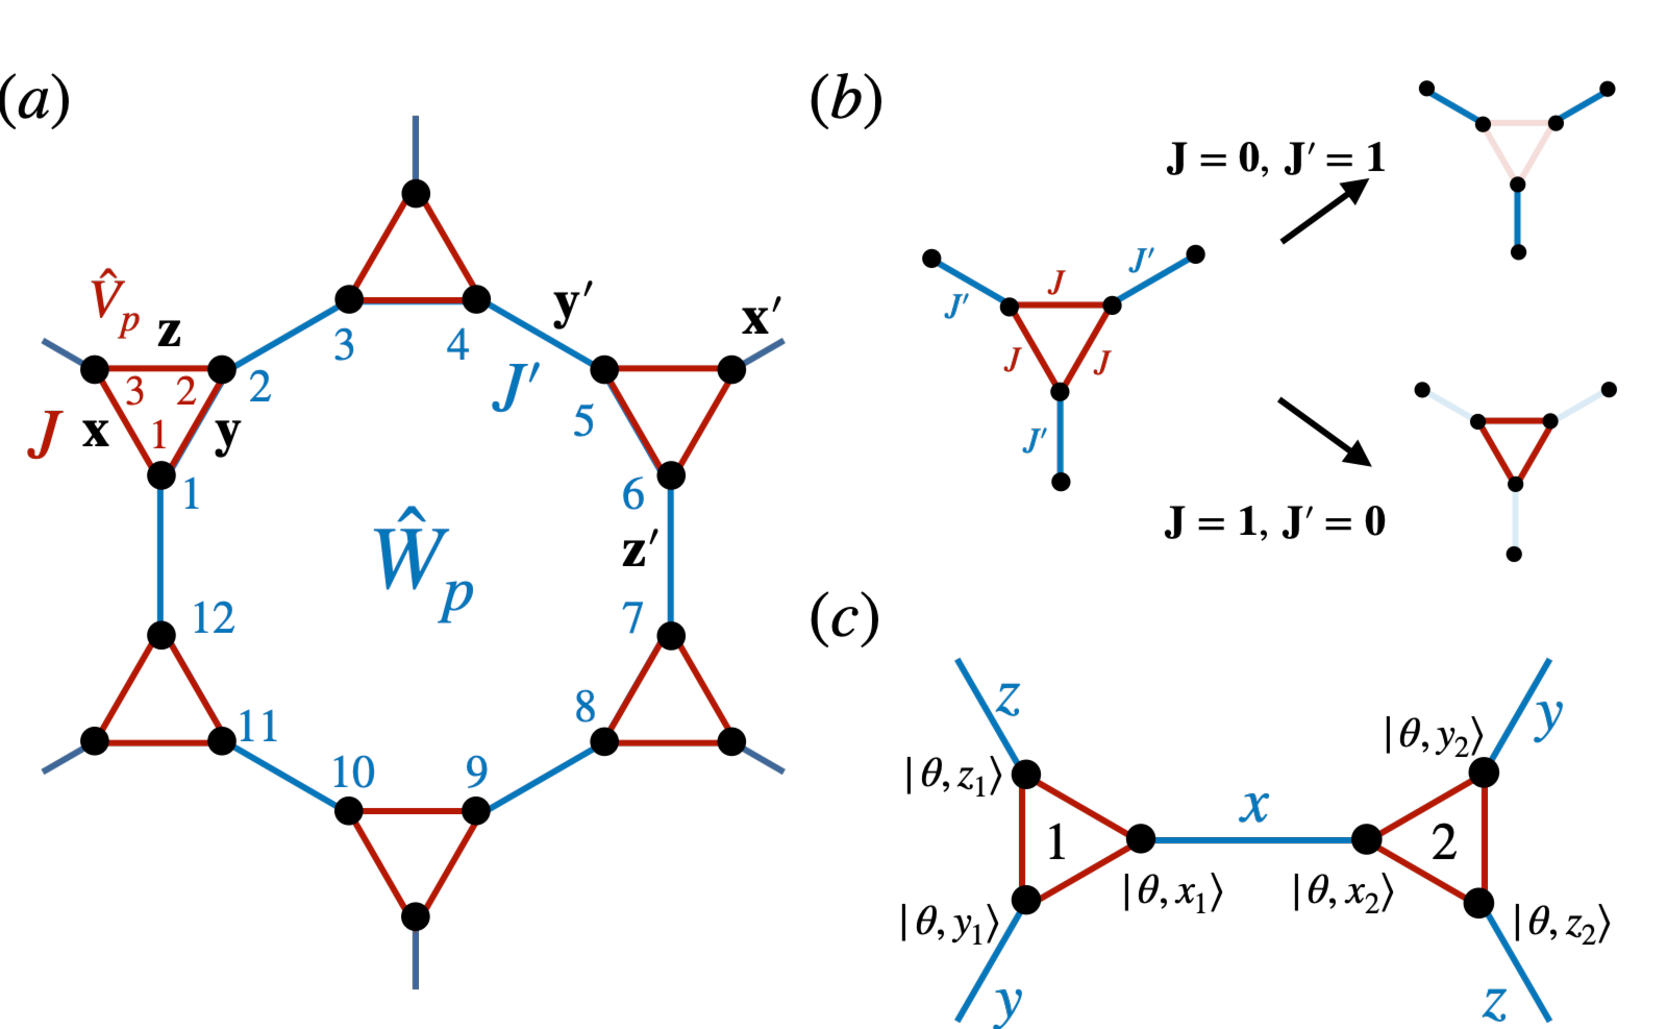
\includegraphics[width=\linewidth]{star_LG}
\caption{ (a) Star lattice with Kitaev-like interactions.  (b) The isolated-dimer and isolated-triangle limits of the Hamiltonian. (c) The initial product state of the LG state.}
\label{fig:star_lattice}
\end{figure}

Let us first consider an LG operator: $\hat{Q}_{\text{LG}} = \text{tTr}\prod_\alpha {Q}^{ss'}_{i_\alpha j_\alpha k_\alpha}|s\rangle \langle s'| $ with the LG tensor defined as
\begin{equation}
Q_{000} = \mathbb{1}, Q_{011} = -iU^x, Q_{101} = -iU^y, Q_{110} = -iU^z.
\end{equation}
where $U^\gamma = e^{i \pi S^\gamma}, \gamma =x,y,z$ is the $\pi$-rotation operator for a given spin (Fig.~\ref{fig:LG_star_tnsr}(a)) ~\cite{lee2020anisotropy}. 
%
One can easily verify that the LG tensor is invariant under the global $\mathbb{Z}_2$ symmetry on the virtual dimension: $Q(u_g \otimes u_g \otimes u_g) = Q $ with $u_g = \mathbb{1}, {\sigma}^z$.
%
 %\textcolor{blue}{YH: I prefer to change previous section (I add $Z_g^{g'} = {(u_Z)}^g \otimes {(u_Z)}^{g'}$), since for LG $u_Z = \sigma^z$ while for SG $u_Z = \sigma^z \otimes I$.}\textcolor{cyan}{YJ: Please make all the symbols consistent.}
Therefore, applying $\hat{Q}_{\text{LG}}$ on any injective PEPS yields a $\mathbb{Z}_2$-injective PEPS. 
%
 $\hat{Q}_{\text{LG}}$ is a projector to the vortex-free space such that $\hat{W}_p\hat{Q}_{\text{LG}} = \hat{Q}_{\text{LG}}\hat{W}_p = \hat{Q}_{\text{LG}}$, $\hat{V}_p\hat{Q}_{\text{LG}} = \hat{Q}_{\text{LG}}\hat{V}_p = \hat{Q}_{\text{LG}}$.
%
Another interesting property of $\hat{Q}_{\text{LG}}$ is that the creation of flux anyon pair discussed in Sec.\ref{sec:Z2-injective} now corresponds to two vortices $W_p = -1$ at the endpoint of the string $u_g^{\otimes L}$ \citep{spin_one_half}.

The LG state can then be obtained by applying $\hat{Q}_{\text{LG}}$ on an initial product state $|\Psi(\theta) \rangle = \otimes_\alpha |\psi_\alpha (\theta) \rangle$ where $\alpha$ is the sites index for a given triangular plaquette and $|\psi_\alpha (\theta)\rangle =  |\theta, x_\alpha \rangle  |\theta, y_\alpha \rangle  |\theta, z_\alpha \rangle$ (Fig.~\ref{fig:star_LG}(c)). 
%
 The magnetic state $ |\theta, \gamma_\alpha \rangle$ satisfies
\begin{equation}
\langle \theta, \gamma| \sigma^{\gamma'}|\theta , \gamma \rangle = \delta_{\gamma' \gamma} \cos \theta + (1-\delta_{\gamma' \gamma})\frac{\sin \theta}{\sqrt{2}}, 
\end{equation}
where $\theta$ is a tunable parameter and $\gamma, \gamma'=x,y,z$.
%
To simplify the notation, we follow the convention in Ref.~\cite{non-AbelianTO_2020} to parametrize the Hamiltonian $H = H(\phi)$ with $J' = \sin(\phi), \ J = \cos(\phi)$. 
%
The ground state for a given Hamiltonian $H(\phi)$ can  then be obtained by variationally optimizing the parameter $\theta$ to find the lowest energy.

To gain more insights, we first consider two limits where the LG state is the exact ground state.  
%
In the isolated-dimer limit,  $H(\phi = \pi/2)$, the  ground state degeneracy is exponentially large with the system size, and one of the ground state basis is a product state $|\Psi \rangle = \otimes_\alpha |\psi_\alpha \rangle$ with $|\psi\rangle = \big( |x,+\rangle | y,+\rangle |z, + \rangle \big)$, where $|\gamma,\pm\rangle$ is the eigenvector of $\sigma^\gamma$ with $\pm 1$ eigenvalues for $\gamma = x,y,z$. 
%
This basis is the initial product state for the LG states with $\theta = 0$ since  $\langle \gamma| \sigma^{\gamma'}| \gamma \rangle = \delta_{\gamma' \gamma}$, and thus one can identify $|\gamma,+\rangle = |\theta = 0, \gamma \rangle$.
%
If we slightly deviate from  $\phi=\pi/2 $, the state is no longer the ground state. 
%
However, we expect the ground state of the model to live in the vortex-free sector, and  
we can apply $\hat{Q}_{\text{LG}}$ to project it back to the vortex-free space,  again giving the LG state at $\theta = 0$.

%\textcolor{blue}{YH: In ~\cite{Hong_Ya_2007}, they show that the ground state live in vortex-free sector for all $J/J' >0$. The isolated-dimer limit should correspond to $J' = 1, J \rightarrow \infty$ but not $J' = 0, J = 1$. In other words, while $J' =0, J = 1$ have exponentially large degeneracies, $J' = \epsilon \ll 1, J = 0$ will only have a specific linear combination of those degenerate grounds states to become vortex free.}
%
Using the fact that $Q_{011}, Q_{101}, Q_{110}$ are  the $\pi$-rotation operator (up to a phase factor) around the $x, y, z$-axes, one can derive the resulting state of the LG operator on $|\theta = 0, \gamma \rangle$ (i.e., $|\gamma,+\rangle$) as in  Fig.~\ref{fig:LG_star_tnsr}(b).
%
Now we can combine three different initial states together to form a triangular product state: $|x,+\rangle |y,+ \rangle |z,+ \rangle $ (Fig. ~\ref{fig:LG_star_tnsr} (c)).
%
For a given set of virtual indices,   the triangular LG state can be written exactly as the sum of two terms due to the $\mathbb{Z}_2$-invariance. 
%
Using the relation in Fig.~\ref{fig:LG_star_tnsr}(b), one can find that the two terms are exactly the same, as shown in Fig.~\ref{fig:LG_star_tnsr}(c). 
%
Furthermore, the physical state with different virtual indices, e.g., $|y,+\rangle,\ |y,- \rangle$ and $|z,+\rangle,\ |z,- \rangle$ in Fig.~\ref{fig:LG_star_tnsr}(c), are orthogonal.
%
This property, combining with the fact the the tensor is $\mathbb{ Z}_2$-invariant, guarantees that the LG state with $\theta = 0$ is $\mathbb{ Z}_2$-isometric~\citep{2011_Norbert_Ginjective}. 
%
Interestingly, the $\mathbb{ Z}_2$-isometry suggest that LG state at $\theta = 0$ is the RG fixed point of $\mathbb{Z}_2$ topological order. 
%
This is consistent with the fact that in the  isolated-dimer limit, the ground state is the same as the that for the TC on the honeycomb lattice ~\citep{KSL_perturbative}. 
%
Note that since SG states is an extension for LG states, it is also $\mathbb{ Z}_2$-isometric at $\phi = \pi/2$. 
%
The property of $\mathbb{ Z}_2 $-isometry allows us to view the toric code with string tension (discussed in Sec.~\ref{sec:Toric Code}) and LG, SG with different parameters on the same footing.


\begin{figure}[tb]
\centering
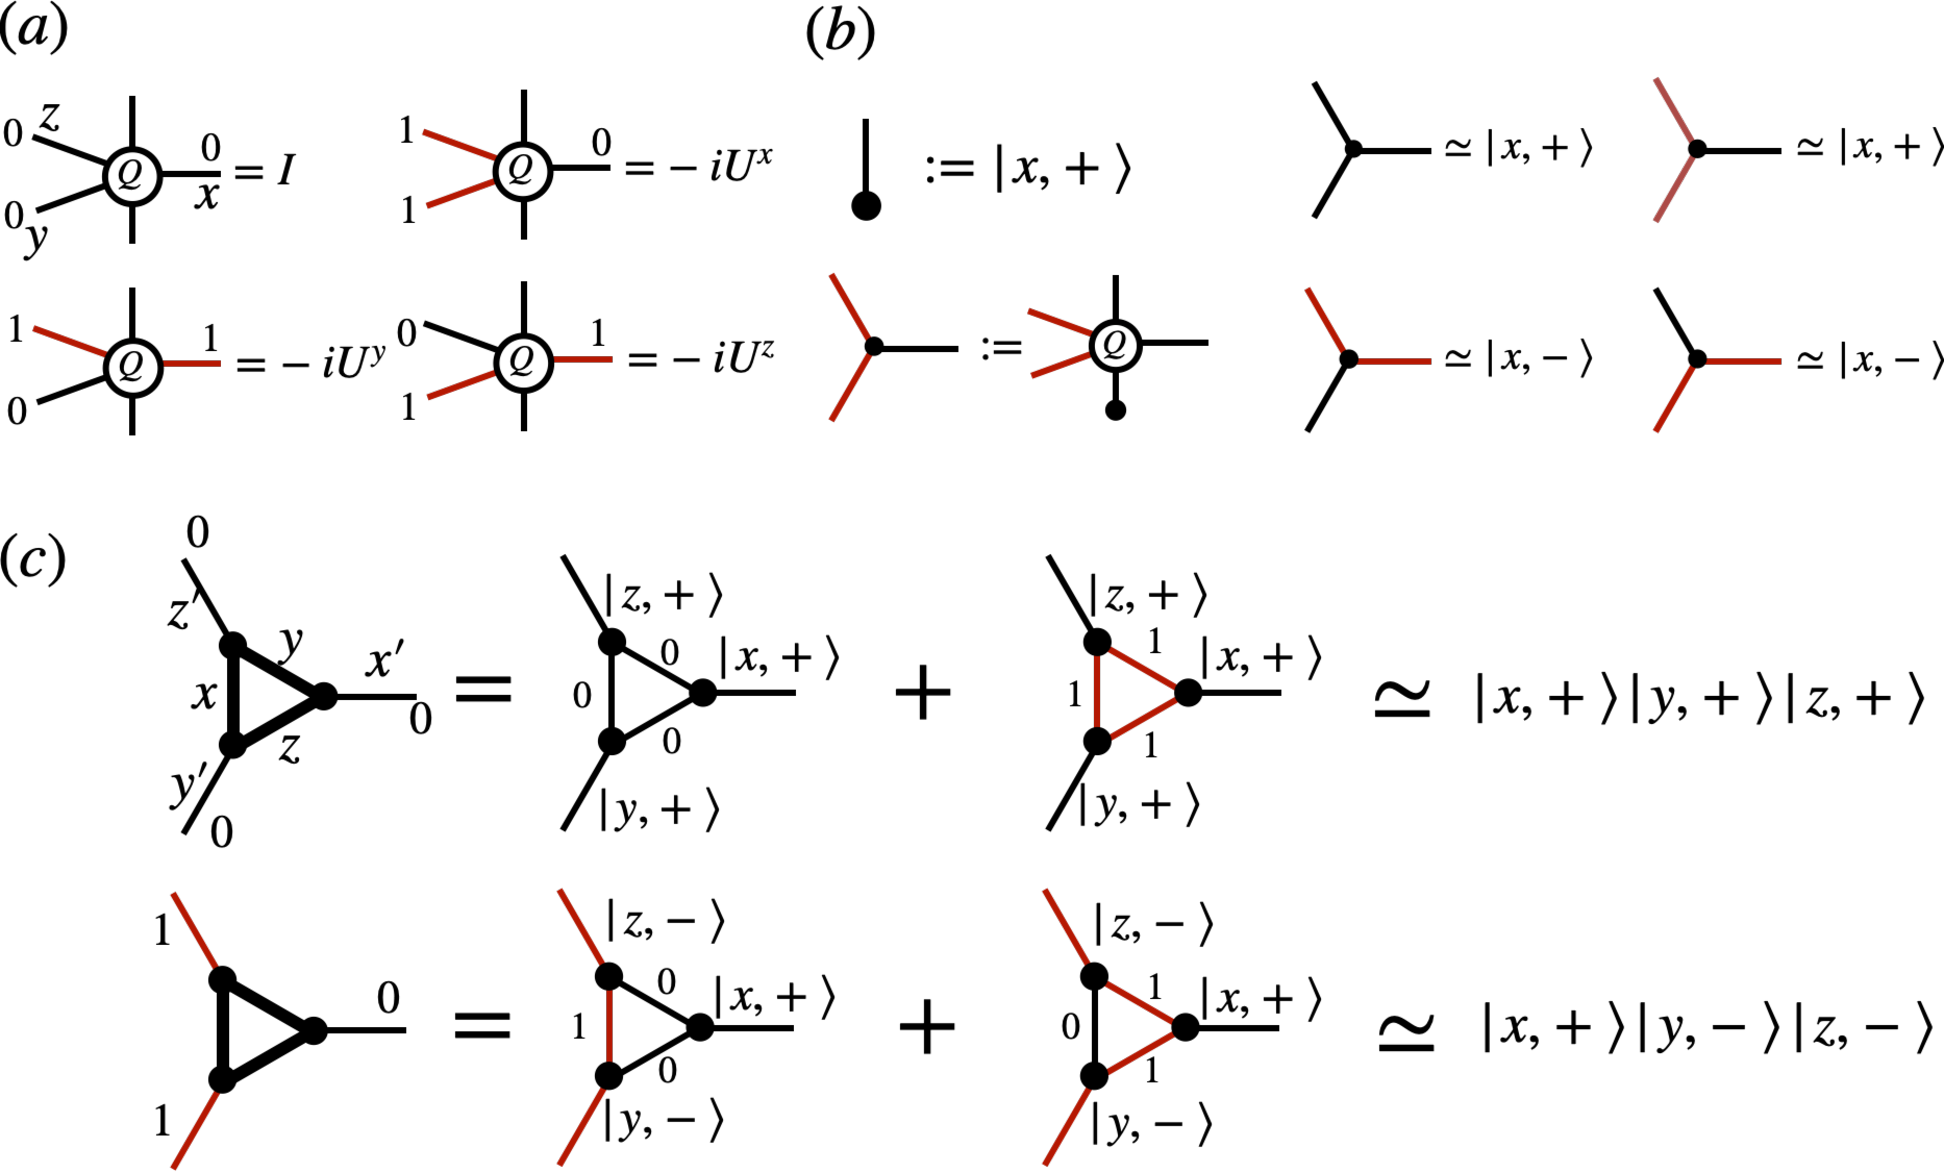
\includegraphics[width=\linewidth]{LG_star_tnsr}
\caption{(a) Non-zero elements of the LG tensor. Here we denote the the virtual index 0(1) as black(red) leg. (b) The resulting states (up to a phase factor) of LG operators acting on $|x,+\rangle$ for a given set of virtual indices. Similar expression can be derived for the initial states $|y(z), +\rangle$.  (c) The resulting states (up to a phase factor) of LG operators acting on $|\psi\rangle=|x,+\rangle |y,+\rangle |z,+\rangle$ for a given set of virtual indices. Here we use the thick lines to denote that the virtual legs are contracted.} 
\label{fig:LG_star_tnsr}
\end{figure}


 

On the other hand, in the isolated-triangle limit, $H(\phi=0)$, the LG state is the exact ground state~\citep{non-AbelianTO_2020,KSL_perturbative}.
%
%The exact energy of the LG states in both limits suggest that they can capture the qualitative feature of the Kitaev star lattice.
%
However, for $0<\phi<\pi$, the energy of the optimized  LG state is higher than the exact value~\cite{non-AbelianTO_2020,Hong_Ya_2007}. 
%
Therefore, instead of using  the optimized LG state for  a specific Hamiltonian $H(\phi)$, in the following we tune the parameter $\theta$ in the  LG state to study its property. 

Similarly, for the SG state, we  introduce the dimer gas (DG) operator $\hat{R}_{\text{DG}}(\alpha, \beta) = \text{tTr}\prod_\gamma {R}^{ss'}_{i_\gamma j_\gamma k_\gamma}(\alpha, \beta)|s\rangle \langle s'| $ with a DG tensor
\begin{equation}
R^{ss'}_{ijk}(\alpha, \beta) = \zeta_{ijk}(\alpha, \beta)[(\sigma^x)^i(\sigma^y)^j(\sigma^z)^k]_{ss'}.
\label{eq:SG}
\end{equation}
where
\begin{equation}
  \zeta_{ijk}(\alpha, \beta)=
    \begin{cases}
      \cos{\beta} & \text{if    } i+j+k = 0\\
      \sin{\alpha} & \text{if    } i+j+k = 1
    \end{cases}.
\end{equation}
%
The SG state can be constructed as $|\psi_\text{SG} (\alpha, \beta)  \rangle = \hat{Q}_\text{LG}\hat{R}_\text{DG}(\alpha, \beta) |\psi(\theta = \tan^{-1}\sqrt2)\rangle$~\cite{non-AbelianTO_2020}.
%
Since the SG state yields quite accurate ground state energy for  the star-lattice Kitaev model, instead of considering  the SG state as a two-parameter family of $\mathbb{ Z}_2 $-injective tensor, we label them using the Hamiltonian parameter $\phi$ instead.


\subsection{Overlap of minimally entangled states}
\label{subsec:overlap of mes}
In the following, we  study the topological properties of the LG and SG states by computing the overlap of MESs, which corresponds to  the dominant eigenvalues of the  TM blocks, $\lambda_{\langle a | b \rangle}$. 
%

As we continuously change the parameter for both the LG and SG states, we find that only the regular and the  TMs measuring the fermion difference (red and green blocks in Fig.~\ref{fig:tm_cylinder}(c)) are non-zero, and there are only four distinct eigenvalues, $\lambda_{\langle I | I\rangle }= \lambda_{\langle \epsilon| \epsilon\rangle} $, $\lambda_{\langle m| m\rangle} = \lambda_{\langle e| e\rangle} $, $ \lambda_{\langle m| e\rangle} = \lambda_{\langle e| m\rangle} $, and $\lambda_{\langle I| \epsilon\rangle} = \lambda_{\langle \epsilon| I\rangle} $, while others are zero. 
%
Therefore, in each category we choose one as the representative.  
% 
Note that since  $\lambda_{\langle I | I \rangle} $ is always the largest, we normalize it to 1. 

Figure~\ref{fig:HOTRG_LG} shows the overlaps of the LG states for $L = 1, 8$, and $256$. 
%
For $L = 1, 8$, we can see that as $\theta$ increase from $0$ to $\theta_c = \cos^{-1}{(2-\sqrt{3})}$, $\lambda_{\langle m| m\rangle}$ gradually decrease and $\lambda_{\langle m| e\rangle}$ gradually increase. 
%
At $\theta = \theta_c$, these two eigenvalues are exactly the same, meaning that we have reached the transition point. 
%

\begin{figure}[t]
\centering
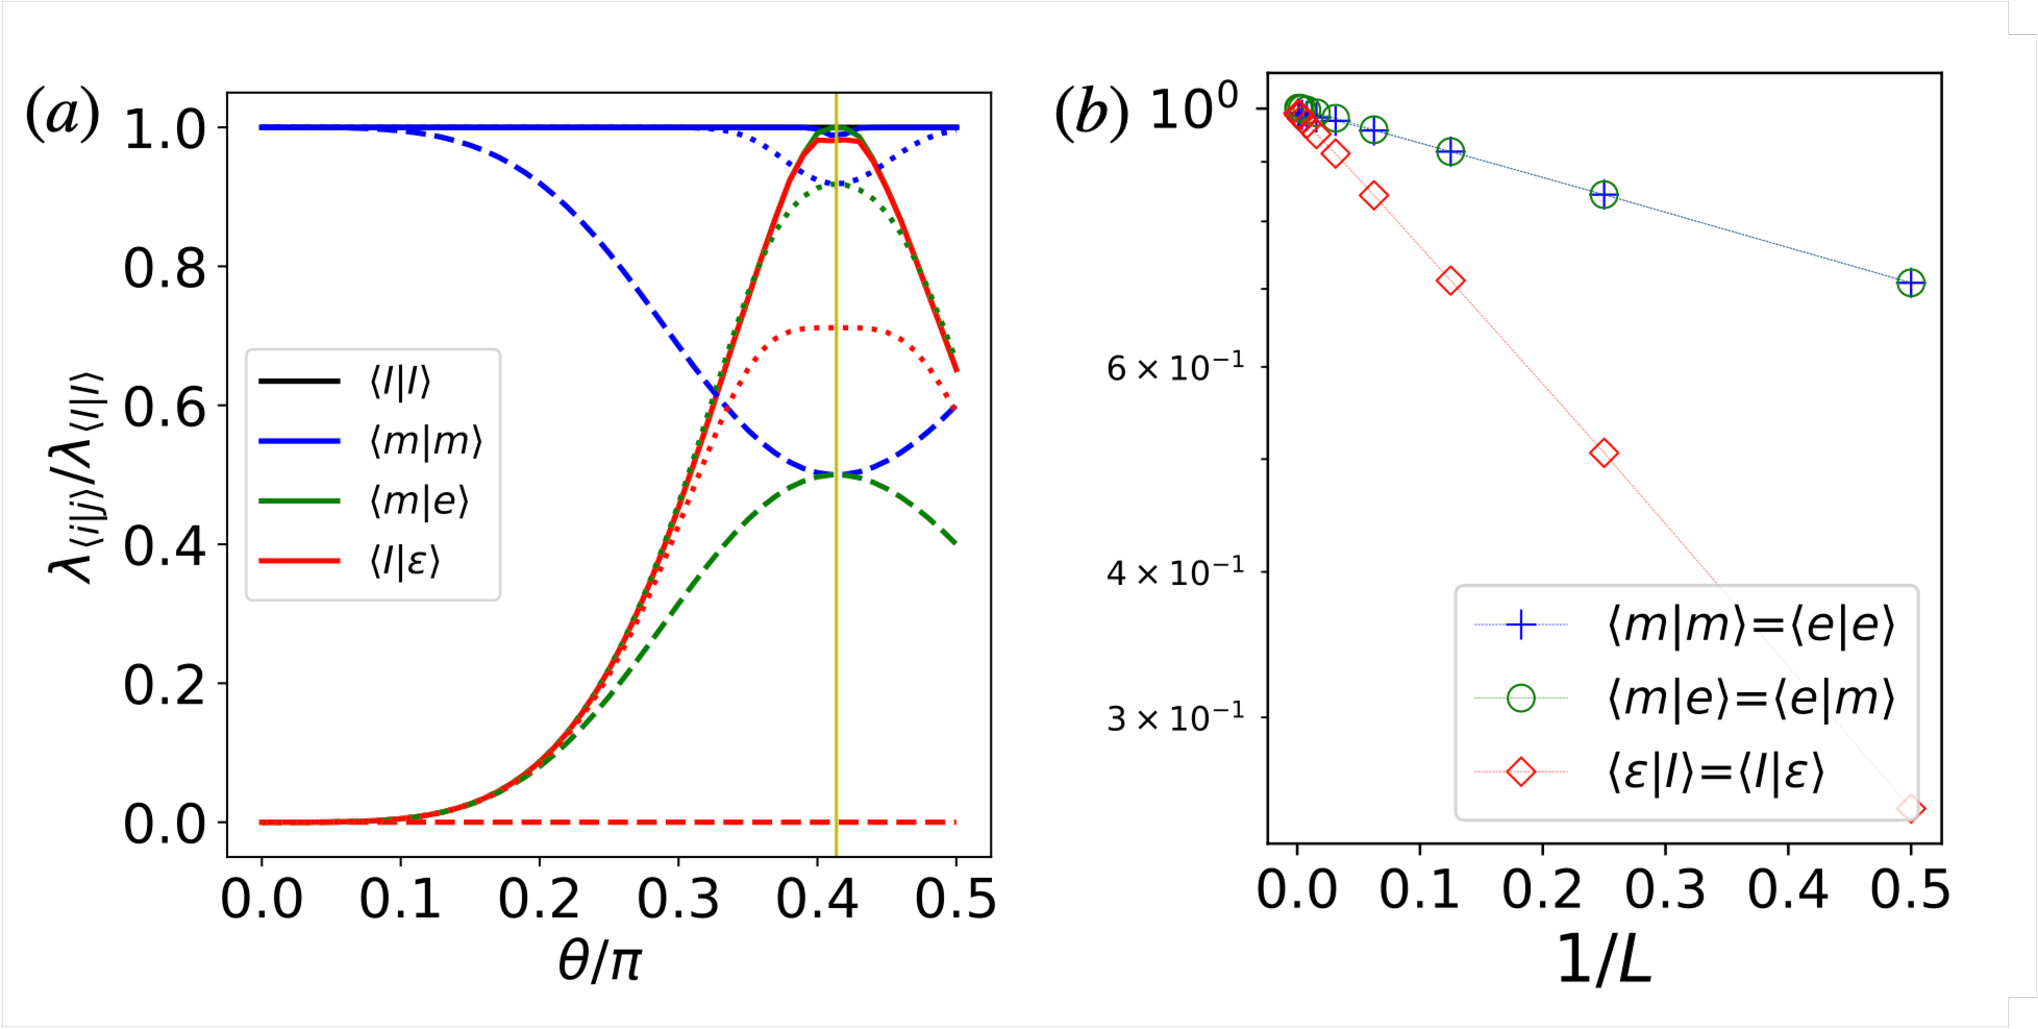
\includegraphics[width=\linewidth]{HOTRG_LG}
\caption{  (a)  Dominant eigenvalues of the transfer matrix for LG states with $L$ = 1 (dashed lines), $L$ = 8 (dotted lines), and $L$ = 256 (solid lines).  (b)  Dominant eigenvalues of the transfer matrix  for $\theta=\theta_c$ with $D_\text{cut} = 80$. }
\label{fig:HOTRG_LG}
\end{figure}


However, if we keep increasing $\theta$, the $\lambda_{\langle m| m\rangle}$ and $\lambda_{\langle m| e\rangle}$ do not cross. 
%
Unlike the level crossing for the charge or flux condensation transition in the toric code with string tension (see Sec.~\ref{sec:Toric Code}), here the dominant eigenvalues for the TM blocks only touch, indicating that $\theta < \theta_c$ and $\theta > \theta_c$ are in the same phase.
%
At  system size $L = 256$, we find that $\lambda_{\langle m| e\rangle} = \lambda_{\langle I| \epsilon\rangle} < 1$ for $\theta \neq \theta_c$. 
%
This means that $\langle m| e\rangle $ and $\langle I| \epsilon\rangle$ should be regarded as the same excitation, and we group them with the same (green) color in Fig.~\ref{fig:tm_cylinder}(c). 
%
Therefore, all the LG states live in the topologically ordered phase, except at $\theta = \theta_c$. 


At the transition point $\theta = \theta_c$, all $\lambda$'s approach   1 as the size increases. 
%
Similar to the transition points studied in Sec.~\ref{sec:Toric Code}, $\lambda_{\langle I| \epsilon\rangle} \to 1$ indicates a gapless excitation; however, we can interpret $\lambda_{\langle m| e\rangle} \to 1$ as  $|e\rangle$ and $|m \rangle$ become the same state..
%
In addition, the spectrum of $\langle m|\epsilon \rangle$ shows no matter how large the system size is, it will  always have two degenerate fixed point; on the other hand, $\langle m|m \rangle$ and $\langle \epsilon|\epsilon \rangle$ have a unique fixed point.
 %
This means that $|m\rangle$ can never be identified with $|\epsilon\rangle$.
 %
We find that $\lambda_{\langle m| e\rangle}$ is always equal to $\lambda_{\langle m| m\rangle} = \lambda_{\langle e| e\rangle}$ regardless of the system size (see Fig.~\ref{fig:HOTRG_LG}(b)). 
 %
This argument can also be supported by the calculation of topological entropy $\gamma$. 
%
We find that both $|e\rangle$ and $|m\rangle$ can yield exactly the same $\gamma = 1/2 \times \ln(2)$ at $\theta = \theta_c$, while $|I\rangle$ and $|e\rangle$ give $\gamma = \ln 2$. 
%
Also, by identifying  $|e\rangle$ with $|m\rangle$, we can explain the three-fold degeneracy of the ground state with the correct total quantum dimension $D = \sqrt{1^2+1^2+(\sqrt{2})^2} = 2$.





To obtain the SG state for each $\phi$, we optimize the free parameters $\alpha$ and $\beta$ in Eq.~\eqref{eq:SG} to obtain the variational ground state of Eq.~\eqref{eq:starKitaev}.
%
Figure~\ref{fig:HOTRG_SG} shows the dominant eigenvalues of the transfer matrices constructed from the SG state. 
%
Recall that the ground state of the star lattice  Kitaev is an Abelian spin liquid at $\pi/3<\phi < \pi$, and non-Abelian at $0<\phi<\pi/3$.
% 
For $\phi = \pi$, the SG state is $\mathbb{ Z}_2 $-isometric just like the LG state at $\theta = 0$. 
%
For $L = 1$, as $\phi$ decreases from $\phi = \pi$ to $\phi \approx 0.24\pi$, $\lambda_{\langle m| m\rangle}$ gradually decreases and $\lambda_{\langle m| e\rangle}$ gradually increases. 
%
At $\phi \approx 0.24\pi$, these two eigenvalues become identical. 
%
Different from the transition in toric code charge condensation, if we keep decreasing $\phi$, both $\lambda_{\langle m| m\rangle}$ and $\lambda_{\langle m| e\rangle}$ increase together.
%
In fact, $\lambda_{\langle m| e\rangle}$ should never become lager than $\lambda_{\langle m| m\rangle}$ since the dominant eigenvalues of the regular transfer matrix will always be larger than other blocks for the norm of the states to stay positive. 
%
However, the trend for $\phi < 0.24\pi$ is also different from the LG case. 
%
The increase of both $\lambda_{\langle m| m\rangle}$ and $\lambda_{\langle m| e\rangle}$ strongly suggest that $|e\rangle$ becomes $|m\rangle$ in that regime. 
%
This is also consistent with the topological entanglement  entropy of $|m\rangle$ becomes $1/2\log(2)$ at $\phi < 0.24\pi$~\cite{non-AbelianTO_2020}. 
%
As $\phi \rightarrow 0$, both $\lambda_{\langle m| m\rangle}$ and $\lambda_{\langle m| e\rangle}$ begin to decrease to the same point as $\phi \approx 0.24 \pi$, suggesting that we have two transition points at $\phi = 0$ and $\phi = 0.24 \pi$. 
%


\begin{figure}[t]
 \centering
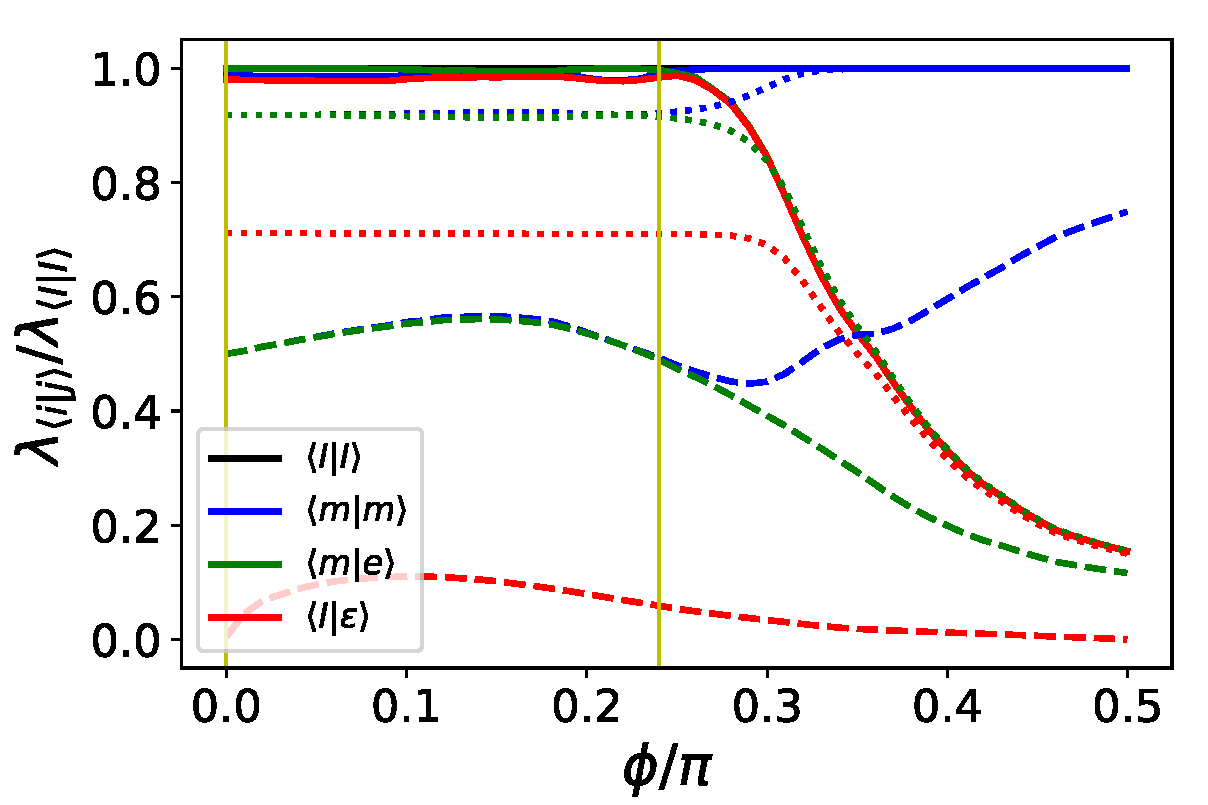
\includegraphics[width=\linewidth]{HOTRG_SG}
\caption{The dominant eigenvalues of the transfer matrices for the SG states with $L$ = 1 (dashed lines), $L$ = 8 (dotted lines), and $L$ = 256 (solid lines).} 
\label{fig:HOTRG_SG}
\end{figure}


As we further increase the circumference to $L = 256$, all $\lambda \rightarrow 1$ for $\phi < 0.24\pi$. 
%
The diverging correlation length suggests that the parent Hamiltonian of the SG states is gapless in this regime.
%
However, as shown in Ref.~\cite{2013_PEPS_chiral_TO}, there might exist other non-frustration-free gapped Hamiltonian, in our case the Kitaev star lattice Hamiltonian, which can also be well approximated by the SG states. 
%
This result is also compatible with  the no-go theorem~\cite{2015_no_go_theorem} that the parent Hamiltonian of  a chiral PEPS is gapless. 
%





\subsection{Transfer Matrix Spectrum}

The full spectrum of the transfer matrices labeled by the momentum quantum numbers can be used to support our picture that $|e\rangle$ and $|m\rangle$ are identical~\citep{Haegeman_2015}. 
%
In Fig.~\ref{LG_thetaC_L6_NA}, we observe that not only the dominant eigenvalues match $\lambda_{\langle e|e\rangle} = \lambda_{\langle m|m\rangle} = \lambda_{\langle m|e\rangle}$, but their full spectra also match. 
%
This means that the two MES $|m\rangle$ and $|e\rangle$ are exactly the same state. 
%
In contrast, while in the thermodynamic limit $\lambda_{\langle I|I\rangle}  = \lambda_{\langle I|\epsilon\rangle} $, their spectra are always different. 
%
This strongly suggests that $\lambda_{\langle e|e\rangle} = \lambda_{\langle m|m\rangle} = \lambda_{\langle m|e\rangle}$ is due to the degeneracy of the state while  $\lambda_{\langle I|I\rangle}  = \lambda_{\langle I|\epsilon\rangle} $ is due to the mode softening.

\begin{figure}[tb]
\centering
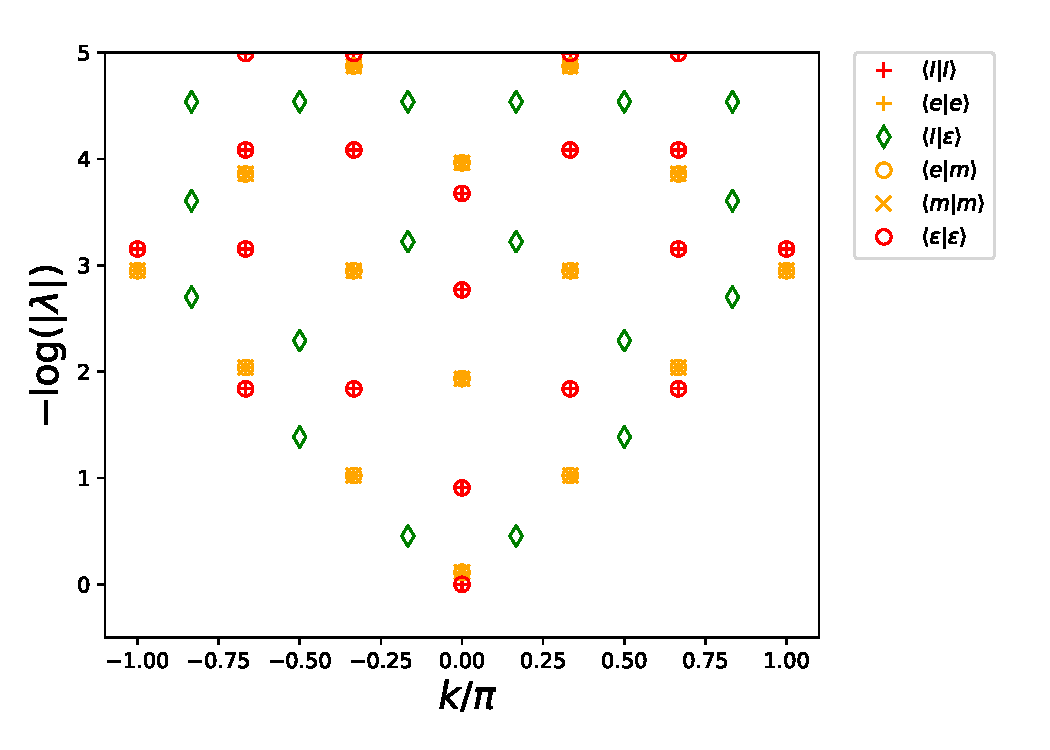
\includegraphics[width=\linewidth]{LG_thetaC_L6_NA}
\caption{ Transfer matrix spectrum of LG at $\theta = \theta_c$ with $L = 6$.} 
\label{LG_thetaC_L6_NA}
\end{figure}

%
Recall the discussion in Sec.~\ref{sec:Toric Code}, once we drive the $\mathbb{Z}_2$-injective wave functions from the TO phase to the CC  phase, the original MES basis is no longer the appropriate basis. 
%
The $|e\rangle$ becomes  exactly the same as $|I\rangle$, and the $|m\rangle$ is not  a physical normalizable state. 
%
Similarly, for the LG and SG states in the non-Abelian regime, there exist no charge and flux anyons anymore. 
%
Combining with the calculation of entanglement entropy in Ref.~\cite{non-AbelianTO_2020}, we can  regard the charge and flux transmute into $\sigma$ anyon for $\phi < 0.24\pi$.
%
 For the honeycomb Kitaev model, the ground state is Abelian when $|J_x| \geq |J_y|+|J_z|$, and the extreme limit can be directly mapped to the TC~\cite{Kitaev2006}. 
%
There, the charge and flux lives in alternating rows of plaquettes. 
%
 On the other hand, in the non-Abelian phase, all the plaquettes should be regarded equal and the vortex excitation is the  $\sigma-$anyon.
 %
Since the Abelian and non-Abelian limit can be respectively mapped to the TC and the isotropic  honeycomb  Kitaev model, there exists a critical point where $|e\rangle$ and $|m\rangle$ transmute into $|\sigma\rangle$.
%
However, the string of $u_g$ and the charge operator $R_\alpha$ encode the fusion and braiding rules for the $\mathbb{Z}_2$ topological order, which can not describe the  non-Abelian case. 
%
This is the limitation of the $\mathbb{Z}_2$ classification built in the $\mathbb{Z}_2$-injective PEPS.
%
As we  show in Sec.~\ref{subsec:overlap of mes}, the parent Hamiltonian is  gapless for $\phi < 0.24\pi$, which does not support gapped $\mathbb{Z}_2$ anyons such as $|e\rangle$ and $|m\rangle$.
%
Within the constraint of the  $\mathbb{Z}_2$-injective PEPS, the best approximate wave function for a non-Abelian CSL is to make $|e\rangle$ and $|m\rangle$ identical.
%
On the other hand, the   star lattice  Kitaev model is \textit{not} the parent Hamiltonian of the SG states  and  excitations can be gapped for $\phi < 0.24\pi$. 
%
This means that the anyonic excitation  described by a $\mathbb{Z}_2$-injective PEPS may not be the true excitation of the model. 
%
Nevertheless, one can create an excitation by the string action $u_g^{\otimes L} = (\hat{\sigma}^z)^{\otimes L}$, which will create a vortex pair with $W_p = -1$ at the endpoints of the string. 
%\input{related}
%\input{photoshoot}
%\input{modeling}
%\input{application}
%\input{conclusion}

\appendix

\backmatter
\phantomsection
\addcontentsline{toc}{chapter}{\bibname}
%\bibliographystyle{abbrv}
\bibliographystyle{ieeetr} 
\bibliography{thesis_v02}

% Your bibliography goes here
%\bibliography{thesis}


\end{document}
